% interacttfssample.tex
% v1.05 - August 2017

\documentclass[]{interact}

\usepackage{epstopdf}% To incorporate .eps illustrations using PDFLaTeX, etc.

%\usepackage[caption=false]{subfig}% Support for small, `sub' figures and tables

%\usepackage[nolists,tablesfirst]{endfloat}% To `separate' figures and tables from text if required

%\usepackage[doublespacing]{setspace}% To produce a `double spaced' document if required
%\setlength\parindent{24pt}% To increase paragraph indentation when line spacing is doubled
%\setlength\bibindent{2em}% To increase hanging indent in bibliography when line spacing is doubled

\usepackage[numbers,sort&compress]{natbib}% Citation support using natbib.sty  %

\usepackage{subfigure}
\usepackage{multirow}
\usepackage{float}
\usepackage{soul}

\graphicspath{{./images/}}


\bibpunct[, ]{[}{]}{,}{}{,}{,}% Citation support using natbib.sty
\renewcommand\bibfont{\fontsize{10}{12}\selectfont}% Bibliography support using natbib.sty

\theoremstyle{plain}% Theorem-like structures provided by amsthm.sty
\newtheorem{theorem}{Theorem}[section]
\newtheorem{lemma}[theorem]{Lemma}
\newtheorem{corollary}[theorem]{Corollary}
\newtheorem{proposition}[theorem]{Proposition}

\theoremstyle{definition}
\newtheorem{definition}[theorem]{Definition}
\newtheorem{example}[theorem]{Example}

\theoremstyle{remark}
\newtheorem{remark}{Remark}
\newtheorem{notation}{Notation}

\begin{document}

%\articletype{ARTICLE TEMPLATE}% Specify the article type or omit as appropriate

\title{Hilbert space methods to approximate Gaussian processes using Stan}

%\author{
%\name{Gabriel Riutort-Mayol, Michael Riis Anderseen, Aki Vehtari, Paul-Christian Burkner}
%\affil{\textsuperscript{a}Department of Cartographic Engineering, Geodesy, and Photogrammetry, Universitat Polit\`ecnica de Val\`encia, Spain; }
%}

\maketitle

\begin{abstract}

\end{abstract}

\begin{keywords}
Gaussian processes; Low-rank Gaussian processes; Hilbert Space methods; Sparse Gaussian processes
\end{keywords}

\tableofcontents


%Contents
\newpage

\section{Introduction}\label{sec:bf_intro}

Gaussian processes (GPs) are natural (Paul: what does "natural" imply and as compared to what?) and flexible non-parametric models to define probability distributions over multi-dimensional functions \citep{rasmussen2006gaussian,neal1997monte}. This allows applying probabilistic inference to estimate functional relationships between one or more covariates and a single response variable. The defining feature of GPs is that the function values are assumed to jointly follow a multivariate normal distribution, which is characterized primarily by a covariance function, sometimes also referred to as covariance kernel. The covariance function encodes our prior assumptions about the functional relationship, such as continuity, smoothness, periodicity and scale properties. GPs not only allow for non-linear effects but can also implicitly handle interactions between covariates. Several types of covariance functions with varying properties can be used, and they may even be combined for further increased flexibility. GPs are often referred to as non-parametric models because the number of parameters is not fixed, but rather increases with the number of data points, which allows to adapt model complexity to the data. As such, the term 'non-parametric' does not imply having no parameters but actually having a lot of them. Due to their generality and flexibility, GPs are of broad interest across machine learning and statistics \citep{rasmussen2006gaussian,neal1997monte}. Among others, they find application in the fields of spatial epidemiology \citep{diggle2013statistical,carlin2014hierarchical}, robotics and control \citep{deisenroth2015gaussian}, signal processing \citep{sarkka2013spatiotemporal}, as well as Bayesian optimization and probabilistic numerics \citep{roberts2010bayesian,briol2015probabilistic,hennig2015probabilistic}.

One of the main limitations of exact GPs is that computational demands and memory requirements scale as $O(n^3)$ and $O(n^2)$, respectively, with the number $n$ of observations in the data used to fit the model. This effectively limits their application to rather small data sets of a few thousand observations at most. This problem becomes especially severe when performing full Bayesian inference via sampling methods, where in each sampling step we need to invert the Gram matrix of the covariance function, usually through Cholesky factorization. To alleviate these computational demands, several approximate methods have been proposed, which we will briefly review in the following. 

Sparse GPs are based on building low-rank approximations of the covariance matrix of the complete data by means of 'inducing variables' (Paul: if you introduce this term, you may need to explain it. Alternatively, can we just get rid of it?). They reduce the dimension of the posterior distribution thereby reducing the memory requirements to $O(nm)$ and computational complexity to $O(nm^2)$ for some $m < n$. This approach still requires Cholesky factorization although now based on a smaller covariance matrix. While computational complexity is reduced considerably, ensuring convergence to the exact GP model is not necessarily straightforward (Paul: this may need a citation). As such, reducing the amount of data while maintaining the correct posterior distribution is not a simple procedure. A unifying view on sparse GPs based on approximate generative methods is provided in \cite{quinonero2005unifying}, while a general review can be found in \cite{rasmussen2006gaussian}. More recent developments in the context of sparse GPs include points-based sparse approximation methods \citep{wilson2015kernel}, which have been further developed by Bui et. al (2017) (Paul: cite this study correctly in latex) to perform approximations at inference time rather than at modeling time.

(Paul: This whole paragraph is unclear to me. Are all of these approaches approximations via splines, or are the splines just special cases of a more general method? In any case, I think the paragraph needs substantial revision). Other global approach make use of the spectral analysis and series expansions of Gaussian processes \citep{loeve1977probability,trees1968detection,adler1981geometry,cramer2013stationary}. It is well-known (see, e.g., \cite{wahba1990spline}) that spline smoothing can be seen as Gaussian process regression with a specific choice of covariance function, but they do not generally have correspondence with GP models, and they do not have the flexibility of choosing different covariance functions as model structure. The Sparse Spectrum GP is based on a sparse approximation to the frequency domain representation of a GP \citep{lazaro2010sparse,quia2010sparse,gal2015improving,gal2015improving}. Recently \citep{hensman2017variational} presented a variational Fourier feature approximation for Gaussian processes that was derived for the Mat´ern class of kernels. Random Fourier Features \citep{rahimi2008random,rahimi2009weighted} is a method for approximating kernels.

Yet another approach to approximate GPs -- on which we will focus in the present paper -- was proposed by \cite{solin2018hilbert} who suggested to use reduced-rank approximations of the covariance kernel. This method decomposes the kernel into basis functions which represent the GP as a linear model and thus makes its estimation considerably faster. In principal, we are free in the choice of basis functions, but the Laplace eigenfunctions were found to be particularily appealing \citep{solin2018hilbert}. Not only can they be computed analytically, but they are also independent of the particular choice of the covariance kernel including the hyperparameters. The latter comes with several advantages when performing inference via algorithms that require differentiation of the posterior density (Paul: cite something here). In a fully Bayesian framework based on sampling methods, the proposed approximate GP model has a computational complexity of just $O(nm+m)$, with $m<<n$ in every sampling step. The posterior distribution of the reduced-rank GP approximation is of dimension $m$ and thus considerably smaller than in the case of exact GPs. This not only lowers the memory requirements but also reduces the correlations between latent values and the corresponding hyperparameters of the GP, which can help to further improve sampling efficiency.

While \cite{solin2018hilbert} fully developed the mathematical theory behind reduced-rank approximations of GPs, they did not put much effort in analyzing the performance and accuracy of the method in relation to key factors such as the number of basis functions, desired prediction space (Paul: I replace 'box size' because, at that point, readers will likely have no idea what that means), or properties of the true functional relationship between covariates and response variable. However, for practical implementations of approximate GPs, the latter factors are critical and thus require further investigation. In the present paper, we will fill this gap by providing practical recommendations for the choice of these factors based on the recognized relations among them. What is more, we provide intuitive visualizations of these relations that will help users to improve performance and save computation time, while at the same time maintaining close approximations of exact GPs. 

Although there are several GP specific software packages available to date (Paul: cite those), each provide efficient implementations only for a restricted range of GP based models. In this paper we do not focus on the fastest possible inference for a specific GP models, but instead are interested in how GPs can be easily used as modular components in probabilistic programming frameworks such as Stan (cite). To this end, we want to make full Bayesian inference over Gaussian process models accessible to a broader audience by making them easy, fast and save to apply. 

The remainder of the paper is structered as follows. In Section 2, we introduce GPs and their reduced rank approximations proposed by \cite{solin2018hilbert}. In Section 3, we analyze the accuracy of these approximations under several conditions using analytical and numerical methods. Several case studies in which we fit
exact and approximate GPs to real and simulated data are provided in Section 4. We end with a discussion in Section 5.

(Paul: The content and the purpose of the following sentences is not fully clear to me. Do we need them in the Introduction or can they be removed, or put into the next section?) While Sparse Spectrum GP is based on a sparse spectrum, the reduced-rank method proposed in this paper aims to make the spectrum as ‘full’ as possible at a given rank. Recent Splines models can reproduce the Matern family of covariance functions (see, e.g., \cite{wood2003thin}), however our approach can reproduce basically all of the stationary covariance functions.

\vspace{3mm}
\section{Method}\label{sec:bf_method}

\subsection{Gaussian process model}

A GP model can be seen as a probability model over an infinite collection of random varibales. However, formally, the defining feature of a GP model is that the joint distribution of function values at any finite number of input values $\mathbf{x}$ is a multivariate normal distribution, 
%
\begin{equation}
f(\mathbf{x}) \sim \mathcal{N}(\mathbf{m},\mathbf{K})
\end{equation}

\noindent with $\mathbf{m}$ the mean vector and $\mathbf{K}$ the covariance matrix. The element $\mathbf{m}_i$ is given by the mean function $m(\mathbf{x}_i)$ and the element $\mathbf{K}_{ij}$ is given by the covariance function $k(x_i,x_j|\theta)$ which is a function of the inputs values $\mathbf{x}$ and the parameters $\theta$. The mean and covariance functions represent how the random functions behave on average and hoe the different points in the input space co-vary with respect to each other:


 In general the mean function $m(\mathbf{x})$ can be any function of the inputs, although this is usually set to zero for simplifying notation. 

\vspace{0.5cm}
\noindent ... \\
... \\
...


\vspace{0.5cm}
A stationary covariance function is a function of $x-x'$, so we can write $k(x,x') = k(x-x')$. Isotropic covariance functions are those that are function of the distance between observations, $k(x,x') = k(|x-x'|) = k(r)$. The Mat\'ern family with half-integers is the class of isotropic covariance functions probably most commonly used, which are
%
\begin{eqnarray}
k_{\nu=\infty}(r)&=&\sigma^2 \text{exp}(-\frac{1}{2} r/\ell^2), \nonumber \\
k_{\nu=\frac{1}{2}}(r)&=&\sigma^2 exp(-r/\ell), \nonumber \\
k_{\nu=\frac{3}{2}}(r)&=&\sigma^2(1+\sqrt{3}r/\ell \text{exp}(-\sqrt{3}r/\ell), \nonumber \\
k_{\nu=\frac{5}{2}}(r)&=&\sigma^2(1+\sqrt{5}r/\ell+\frac{5}{3}r^2/\ell^2) \text{exp}(-\sqrt{5}r/\ell), \nonumber 
\end{eqnarray}

\noindent where $\nu$ is the order the kernel, and the $\ell$ and $\sigma$ are the lengt-scale and magnitud, respectively, of the kernel. The particular case where $\nu=\infty$ is commonly known as squared exponential (exponentiated quadratic) covariance function, and that with $\nu=1/2$ as exponential covariance function. These covariance functions can be easily generalized to the multidimensional case considering multidimensional inputs $\mathbf{r}$ and the multidimensional length-scale $\boldsymbol{\ell}$. 

The spectral density functions associated with the univariate Mat\'ern covariance functions written above are
%
\begin{eqnarray}
S_{\nu=\infty}(w)&=& \sigma^2 \sqrt{2\pi} \cdot \ell \cdot \text{exp}(-0.5 \ell^2 w^2), \nonumber \\
S_{\nu=\frac{1}{2}}(w)&=& 2\sigma^2 \frac{1}{\ell}(\frac{1}{\ell^2} + \omega^2)^{-1}, \nonumber \\
S_{\nu=\frac{3}{2}}(w)&=& 4\sigma^2 \frac{\sqrt{3}}{\ell}^{3}(\frac{3}{\ell^2} + \omega^2)^{-2}, \nonumber \\
S_{\nu=\frac{5}{2}}(w)&=& \frac{16}{3}\sigma^2 \frac{\sqrt{3}}{\ell}^{5}(\frac{5}{\ell^2} + \omega^2)^{-3}, \nonumber 
\end{eqnarray}

\noindent where variable $w$ is in the frequency domain.


\subsection{Hilbert space-based approximate Gaussian process model}

The approximate Gaussian process method, developed by \cite{solin2018hilbert} and implemented in this paper, lay on the basis of considering the covariance operator of a homogeneous (stationary) covariance function as a pseudo-differential operator constructed as a series of Laplace operators. Then, the pseudo-differential operator is approximated with Hilbert space methods on compact subsets $\Omega \subset {\rm I\!R}^D$, and with some boundary condition. 

First, we focus on the unidimensional case of the input space, such as $\Omega \in \{-L,L\} \subset {\rm I\!R}$, where $L$ is some positive real value. 

\vspace{0.2cm}
The approximate method leads to the approximation of the covariance function between two input values $\{x,x'\} \in \{-L,L\}$ as 
%
\begin{equation}\label{approxcov}
k(x,x') \approx \sum_{j}S_{\theta}(\sqrt{\lambda_j}) \phi_j(x) \phi_j(x'),
\end{equation} 

\noindent where $S_{\theta}$ is the spectral density of the stationary covariance function $k$ and $\theta$ the set of hyperparameters of $k$; a stationary covariance function can be equivalently represented in terms of the spectral density \citep{rasmussen2006gaussian}, then the spectral density is a function of the hyperparameters $\theta$. $\{\lambda_j\}_{j=1}^{\infty}$ and $\{\phi_j(x)\}_{j=1}^{\infty}$ are the set of eigenvalues and eigenvectors, respectively, of the Laplacian operator. Namely, they satisfy the following eigenvalue problem in the compact subset $x \in \{-L,L\}$ and with the Dirichlet boundary condition (another boundary condition could be used as well):
%
\begin{eqnarray}\label{eigenproblem}
-\nabla^2 \phi_j(x)&=&\lambda \phi_j(x), \hspace{1cm}  x\in \{-L,L\} \nonumber \\ 
\phi_j(x)&=&0, \hspace{2cm} x\notin \{-L,L\}.
\end{eqnarray} 

\noindent The eigenvalues $\lambda_j>0$ are real and positive, because the Laplacian is a positive definite Hermitian operator, and the eigenfunctions $\phi_j$ for the eigenvalues problem in eq. (\ref{eigenproblem}) are sinusoidal functions,
%
\begin{eqnarray}
\lambda_j&=&\left(\frac{j\pi}{2L}\right)^2, \\
\phi_j(x)&=&\sqrt{\frac{1}{L}} \text{sin}\left(\sqrt{\lambda_j}(x+L)\right).
\end{eqnarray}

If we truncate the sum in (\ref{approxcov}) up to $J$ ($j=1,\cdots,J$), the approximate covariance function can be represented as
%
\begin{equation}
k(x,x') \approx \boldsymbol{\phi}(x)^\intercal \Delta \boldsymbol{\phi}(x'), \nonumber
\end{equation}

\noindent where $\boldsymbol{\phi}(x)=\{\phi_j(x)\}_{j=1}^{J} \in {\rm I\!R}^{J}$ is the column vector of basis functions, and $\Delta  \in {\rm I\!R}^{J\times J}$ the diagonal matrix of espectral densities $S_{\theta}(\sqrt{\lambda_j})$, 
%
\begin{eqnarray}
\Delta &=&  \begin{bmatrix}
    S_{\theta}(\sqrt{\lambda_1}) & & \\
    & \ddots & \nonumber \\
    & & S_{\theta}(\sqrt{\lambda_J}) \\
  \end{bmatrix}.
\end{eqnarray}

Thus, the Gram matrix $\text{K}$ of the covariance function $k$ for a collection of observations $i=1,\cdots,N$ and collection of input values $\{x^i\}_{i=1}^{N} \in {\rm I\!R}^{N}$ can be represented as follows
%
\begin{equation}
\text{K}= \Phi \Delta \Phi^\intercal, \nonumber
\end{equation}

\noindent where $\Phi \in {\rm I\!R}^{N\times J}$ is the matrix of eigenfunctions $\phi_j(x^i)$,
%
\begin{eqnarray}
\Phi &=&  \left[ {\begin{array}{ccc}
   \phi_1(x^1) & \cdots & \phi_J(x^1)  \\
    \vdots &\ddots & \vdots  \nonumber \\ 
    \phi_1(x^N) & \cdots & \phi_J(x^N) \\
  \end{array} } \right].
\end{eqnarray}
 
\noindent Now, the Gaussian process prior for the function $f$ can be re-defined as
%
\begin{equation}
\mathbf{f} \sim \text{GP}(0,\Phi \Delta \Phi^\intercal). \nonumber
\end{equation}

\noindent This equivalently leads to a linear representation of the function $f$,
%
\begin{equation}\label{approxf}
f(x) \approx \sum_{j} \left( S_{\theta}(\sqrt{\lambda_j})\right)^{1/2} \phi_j(x) \beta_j, \nonumber
\end{equation}

\noindent where $\beta_j \sim \text{N}(0,1)$ is a random variable with zero mean and unitary variance. That is, the function $f$ can be approximated with a finite basis function expansion (eigenfunctions $\phi_j$ of the Laplace operator), scaled by the squared root of the spectral density as a function of the eigenvalues $\lambda_j$. The eigenfunctions $\phi_j$ do not depend on the kernel hyperparameters $\theta$, the only dependence on $\theta$ is through the spectral density $S_{\theta}$. The eigenvalues $\lambda_j$ are monotonically increasing with $j$ and the spectral density goes rapidly to zero for bounded covariance functions. Therefore, it is expected a good approximation in eq. (\ref{approxf}) for a finite number, $J$, of terms in the series as long as the inputs values $x^i$ are not near the boundaries of the domain $[-L,L]$, where the Laplacian was taken to be zero.

The computational cost of this approximate model scales $O(n\cdot J+J)$, where $n$ is the number of observations and $J$ the number of basis functions.



\subsection{Generalization to multidimensional input space}

We are going to generalize the results from the previous section to a multidimensional input space with compact regular domain $\Omega=[-L_1,L_1] \times \dots \times [-L_d,L_d]$ and Dirichlet boundary conditions. We assume the same number $J$ of basis functions terms in the series expansion for every input dimension, however it is straight forward to generalize this to different number of term series $J_d$ for every dimension. 

\vspace{0.2cm}
In a $D$-dimensional input space the total number of eigenfunctions and eigenvalues in the approximation corresponds to the total number of $D$-tuples over $J$, which is $J^D$. Let $\mathbb{S}\in {\rm I\!R}^{J^D \times D}$ be the set of $D$-tuples elements. Each new eigenfunction $\phi^{\ast}_j$ correspond to the product of the univariate eigenfunctions whose indices corresponds to the the elements of the $D$-tuple $\mathbb{S}_{j\cdotp}$. And each new eigenvalue $\lambda^{\ast}_j$ is a $D$-vector whose elements are the univariate eigenvalues whose indices correspond to the elements of the $D$-tuple $\mathbb{S}_{j\cdotp}$. Let $j=\{1,\cdots,J^D\}$,
%
\begin{eqnarray}
\phi^{\ast}_j(\mathbf{x}) &=& \prod_{d=1}^{D} \phi_{\mathbb{S}_{jd}}(\mathbf{x}_d) = \prod_{d=1}^{D} \sqrt{\frac{1}{L_d}} \text{sin}\left(\sqrt{\lambda_{\mathbb{S}_{jd}}}(\mathbf{x}_d+L_d)\right)  \nonumber \\
%
\lambda^{\ast}_j &=& \{\lambda_{\mathbb{S}_{jd}} \}_{d=1}^D =  \{ \left(\tfrac{\pi \mathbb{S}_{jd}}{2L_d}\right)^2 \}_{d=1}^D  \nonumber
\end{eqnarray}

As an example we show the matrix $\mathbb{S}$ for a $three$-dimensional input vector $\mathbf{x}=\{\mathbf{x}_1,\mathbf{x}_2,\mathbf{x}_3\}$ ($D=3$) and $J_{1}=2$, $J_{2}=2$ and $J_{3}=3$ eigenfunctions and eigenvalues for the first, second and third dimensions, respectively. The number of new multidimensional eigenfunctions $\phi^{\ast}$ and eigenvalues $\lambda^{\ast}$ is $J_{1}\cdot J_{2}\cdot J_{3}=2\cdot 2\cdot 3=12$. The matrix $\mathbb{S}\in {\rm I\!R}^{12 \times 3}$ is
%
\begin{eqnarray}
\mathbb{S}=
\left[ {\begin{array}{ccc}
1 & 1 & 1 \nonumber \\
1 & 1 & 2 \\
1 & 1 & 3 \\
1 & 2 & 1 \\
1 & 2 & 2 \\
1 & 2 & 3 \\
2 & 1 & 1 \\
2 & 1 & 2 \\
2 & 1 & 3 \\
2 & 2 & 1 \\
2 & 2 & 2 \\
2 & 2 & 3 
\end{array} } \right]
\end{eqnarray} 


The approximate covariance function is represented as
%
\begin{equation}\label{approxcov_multi}
k(\mathbf{x},\mathbf{x}') \approx \sum_{j=1}^{J^D} S^{\ast}_{\theta}\left(\sqrt{\lambda^{\ast}_j}\right) \phi^{\ast}_j(\mathbf{x}) \phi^{\ast}_j(\mathbf{x}'),
\end{equation}

\noindent where $S^{\ast}_{\theta}$ is the spectral density of the $D$-dimensional covariance function. The $D$-dimensional spectral density functions associated with the Mat\'ern covariance functions considered in the previous section are
%
\begin{eqnarray}
S^{\ast}_{\nu=\infty}(\mathbf{w})&=& \sigma^2 \sqrt{2\pi}^D \prod_{d=1}^D l_d \cdot \text{exp}\left(-0.5 \sum_{d=1}^D l_d^2 \mathbf{w}_d^2\right), \nonumber \\
%
S^{\ast}_{\nu}(\mathbf{w})&=& \frac{2^D\pi^{D/2}\Gamma(\nu+D/2)(2\nu)^{\nu}}{\Gamma(\nu)l^{2\nu}}\left(\frac{2\nu}{l^2}+4\pi^2\mathbf{w}^2 \right)^{(\nu+D/2)}, \nonumber
\end{eqnarray}

\noindent where the $D$-vector $\mathbf{w}$ is in the frequency domain. We can represent the approximate series expansion of the function $f$ in the multidimensional input space as,
%
\begin{equation}\label{approxf}
f(\mathbf{x}) \approx \sum_{j} \left( S^{\ast}_{\theta}(\sqrt{\boldsymbol{\lambda^{\ast}_j}})\right)^{1/2} \phi^{\ast}_j(\mathbf{x}) \beta_j, 
\end{equation}

\noindent where $\beta_j \sim \text{N}(0,1)$ is a random variable with zero mean and unitary variance. The computational cost in a multidimensional setting scales $O((n+1)\cdot \prod_{d=1}^D J_d )$, where $n$ is the number of observations and $J_d$ is the number of basis functions considered in the dimension $d$.

\subsection{Learning hyperparameters and model inference}

\vspace{2mm}
$\bullet$ It has an attractive computational cost as this basically turns the regular GP model into a lineal model.

\vspace{2mm}
$\bullet$ The design matrix of the proposed linear model, which is composed of a basis of Laplace eigenfunctions, can be computed analytically and does not depend on the hyperparameters of the model, then it has to be computed only once with $O(n+m)$ computational demands.

\vspace{2mm}
$\bullet$ The weights associated to the basis functions in this linear model is a $m$-dimensional vector ($m$ is the number of basis functions) and their computation is an operation with $O(m)$ computational demands. The weights depend on the hyperparameters, then they have to be computed in every step of the HMC sampling method.

\vspace{2mm}
$\bullet$ The linear model is computed with complexity $O(nm)$, computed in every step of the HMC sampling method.

\vspace{2mm}
$\bullet$ In a fully Bayesian inference framework using sampling methods, the proposed approximate GP model has a computational complexity of $O(nm+m)$ in every step of the HMC method. In addition, the computation of the automatic differentation to compute the gradients in this linear model scales $O(n)$?, an operation that must be computed in every step of the HMC method.

\vspace{2mm}
$\bullet$ Using maximizing marginal likelihood methods, the proposed model has a overall complexity of $O(nm^2)$. After this, evaluating the marginal likelihood and marginal likelihood gradients is an $O(m^3)$ operation in every step of the optimizer. (Arno's paper, pag. 7)

\vspace{2mm}
$\bullet$ The parameter posterior distribution in this approximate GP model is $m$-dimensional ($m<<n$) which helps the use of GP priors as latent functions. especially when sampling methods for inference are used. GP prior as latent functions is needed in generalized models.

In regular GPs and other approximate GP models and Splines models these features do not have so nice properties:

\vspace{2mm}
$\bullet$ In a regular GPs, the main computational complexity comes from the inversion of the covariance matrix which is in general a $O(n^3)$ operation. This operation has to be computed at every step of the HMC or optimizer.

\vspace{2mm}
$\bullet$ In regular GPs, the parameter posterior distributions is $N$-dimensional. It is known that when $N$ is of medium or large size there is high correlation between the $N$-dimensional latent function and the hyperparameters of the GP prior.

\vspace{2mm}
$\bullet$ In conventional sparse GP approximations, although the rank of the GP is reduced considerably to the number of inducing points, this still needs to do the autodiff and covariane matrix inversion.

\vspace{2mm}
$\bullet$ The Splines models are also a sort of basis functions expansion model, then the computational demands are similar to that in this approach. However in Splines models the lengthscale hyperparameter tend to be fixed and then the fit is covered by the magnitud parameter. In that sense, Splines models tend to loose the useful interpretation of the lengthscale parameter.

\vspace{2mm}
$\bullet$ In addition, the computation of the automatic differentation to compute gradients in this linear model scales $O(n)$, which is an operation that must be computed in every step of the HMC method.

\vspace{2mm}
$\bullet$ In a regular GP model the automatic differentation to compute the gradients of the covariance function scales $O(n^2)$, the dimension of the covariance matrix, and the full inversion of the covariance matrix scales $O(n^3)$. This operation has to be computed at every step of the HMC.

\vspace{2mm}
$\bullet$ In a sparse GP approach based on inducing points, although the rank of the GP is reduced considerably to the number of inducing points, this still needs to do the autodiff and covariane matrix inversion.

\vspace{2mm}
$\bullet$ The Splines models are also a sort of basis functions expansion model, then the computational demands are similar to that in this approach.


\section{The accuracy of the approximation}

The performance and accuracy of the method are directly related with the number of basis functions and the box size, and, at the same time, these two factors depend on the smoothness or roughness of the process. The time of computation is mainly dependent on the number of basis functions. Our main contributions to this recently developed methodology for low-rank GP model by \cite{solin2018hilbert} goes around these aspects.

\vspace{2mm}
$\bullet$ We investigate the relations going on among these factors, the number of basis functions, the box size, and the lengthsccale of the function.

\vspace{2mm}
$\bullet$ We make recomendations for the values of these factors based on the recognized relations among them. We provide useful graphs of these relations that will help the users to improve performance and save time of computation.

\vspace{2mm}
$\bullet$ We also diagnose if the chosen values for the number of basis functions and the box size are adequate to fit to the actual data.


\subsection{Dependency on the number of basis functions and the boundary condition}

The approximation of the covariance function is a series expansion of eigenfunctions and eigenvalues of the Laplace operator in a given domain $\Omega$, e.g. in a 1-$D$ input space $x\in \Omega=[-L,L]$:
%
\begin{equation}\label{diffcov}
k(\tau) \approx \sum_{j}S_{\theta}(\sqrt{\lambda_j}) \phi_j(\tau) \phi_j(0),  \nonumber
\end{equation} 

\noindent where $j$ is the index for the eigenfunctions and eigenvalues, and $\tau=x-x'$. The eigenvalues $\lambda_j$ and eigenfunctions $\phi_j$ are 
%
\begin{eqnarray}
\lambda_j&=&\left(\frac{j\pi}{2L}\right)^2, \nonumber \\
\phi_j(x)&=&\sqrt{\frac{1}{L}} \text{sin}\left(\sqrt{\lambda_j}(x+L)\right). \nonumber
\end{eqnarray} 

The approximation to the covariance function will become exact in the limit when the number of basis functions approach infinity $J=1,\dots,j,\dots,\infty$. The number of basis functions can be truncated that the difference between the covariance function and the approximation be less than a threshold $\epsilon$,
%
\begin{eqnarray}\label{diff_covs}
\int k(\tau)d(\tau) - \int \sum_{j}S_{\theta}(\sqrt{\lambda_j}) \phi_j(\tau) \phi_j(0) d(\tau) < \epsilon.
\end{eqnarray}

The finite number of basis functions in the approximation to satisfy eq. (\ref{diff_covs}) will depend on the smoothness or roughness of the function, that is, on the lengthscale $\ell$. The approximation will also depends on the box size $L$ which will affect the performance specially near the boundaries. 

To illustrate the effects of these two factors, number of basis functions $J$ and box size $L$, on the performance of the approximation, let's consider a simulated dataset of 75 noisy observations from a GP prior with lengthscale $\ell=0.3$ and magnitud $\alpha=1$. The additive noise added to the GP prior simulations is $\sigma=0.2$. A regular GP model and different approximate GP models with different choices for the number of basis function $J$ and box size $L$ are fitted on this dataset. 

For a fixed $L$, let's suppose it is set to a right choice, Figure \ref{image2_J} shows the effect of the number of basis functions in approaching the posterior mean and the covariance function. The number of basis functions affects the non-linearity or roughness (or smoothness) of the posteriors. Fewer basis functions implies smoother covariance functions and consequently smoother posteriors. The more roughness the process is, the more basis functions are needed. 

\begin{figure}[H]
\centering
\subfigure{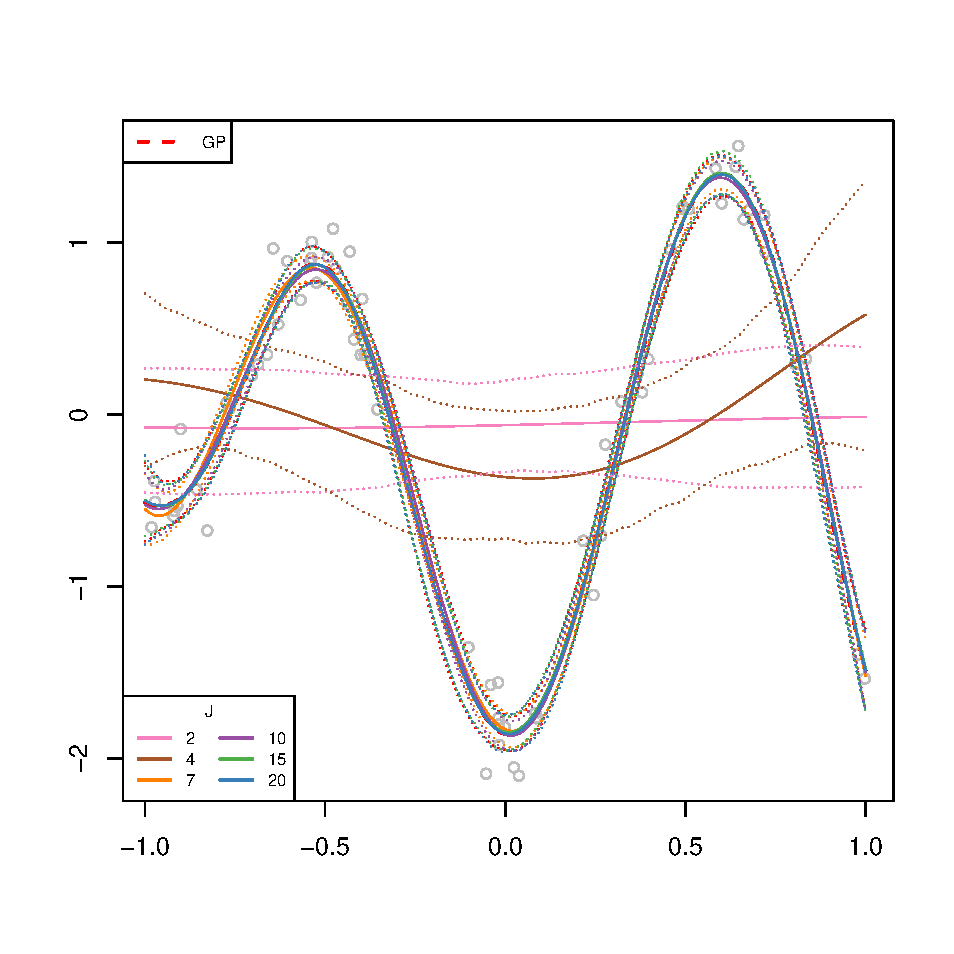
\includegraphics[scale=0.4, trim = 0mm 0mm 0mm 10mm, clip]{fig1_Post_J.pdf}}
\subfigure{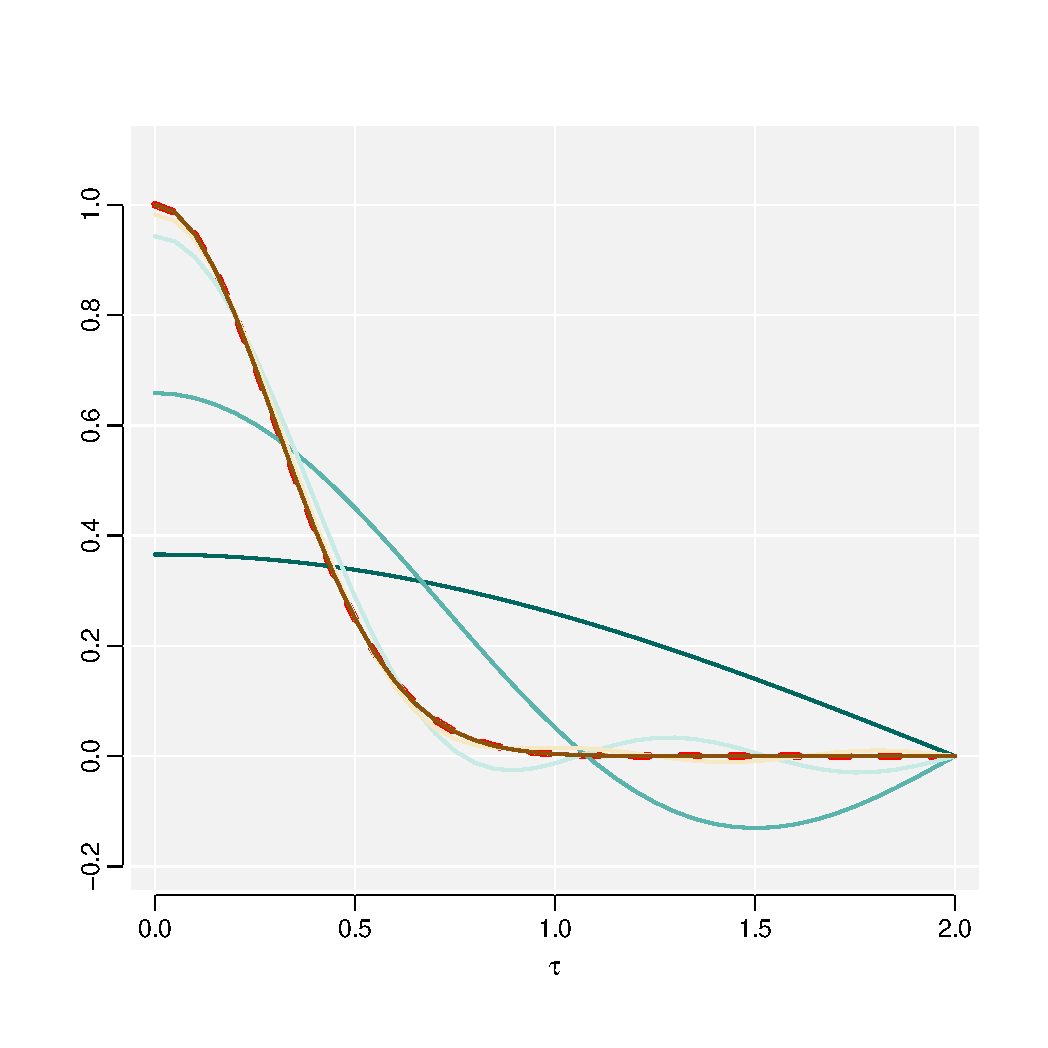
\includegraphics[scale=0.4, trim = 0mm 0mm 0mm 10mm, clip]{fig1_Cov_J.pdf}}
\caption{(left) Posterior distributions for different number of basis functions $J$. (right) Covariance function for different number of basis functions $J$.}
  \label{fig1_Post_J}
\end{figure}

Similarly, for a fixed number of basis functions $J$, let's suppose it is set to a right choice, Figure \ref{fig2_Post_L} shows the effect of the box size $L$ in approaching the posterior mean and the covariance function. The box size mainly affects the approximation near the boundaries of the function, and affects the covariances at long distances.

\begin{figure}[H]
\centering
\subfigure{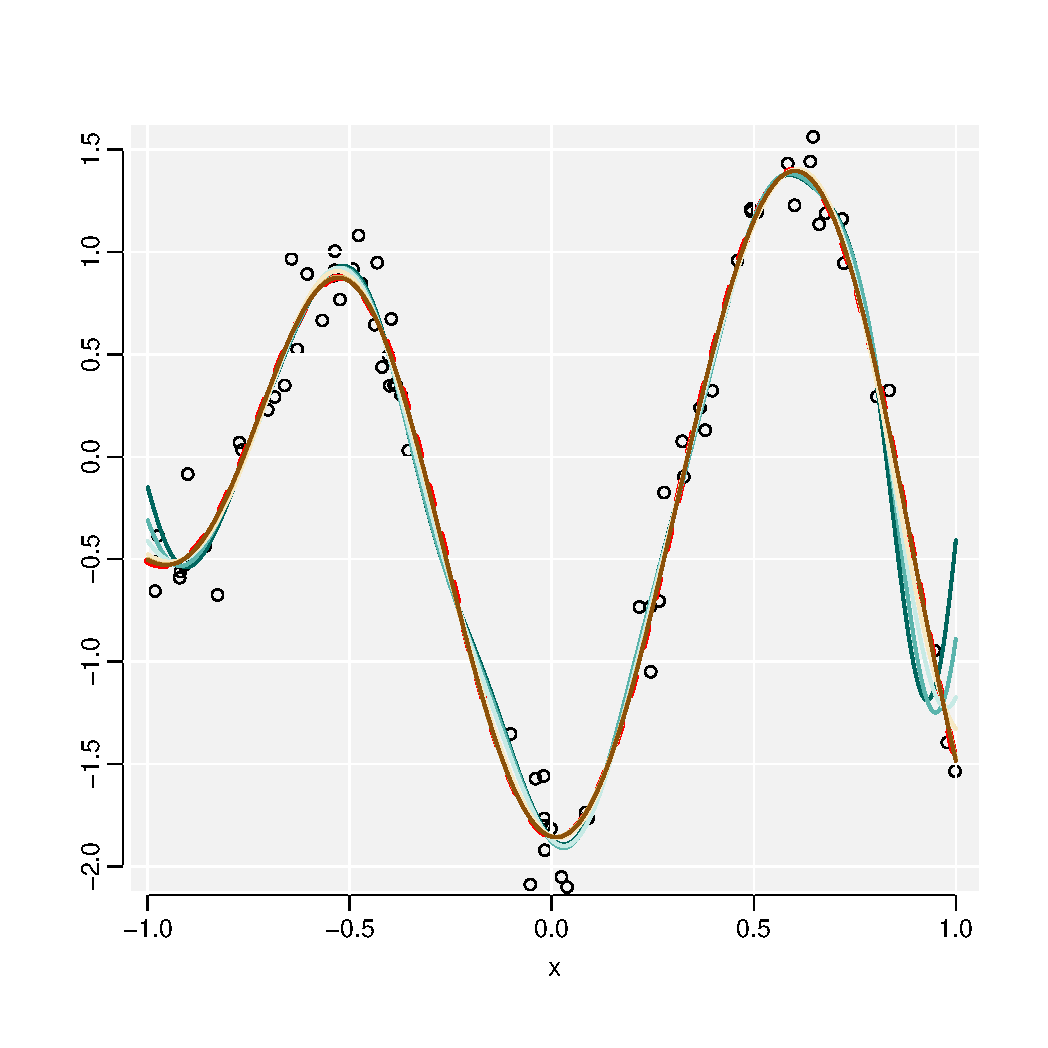
\includegraphics[scale=0.4]{fig2_Post_L.pdf}}
\subfigure{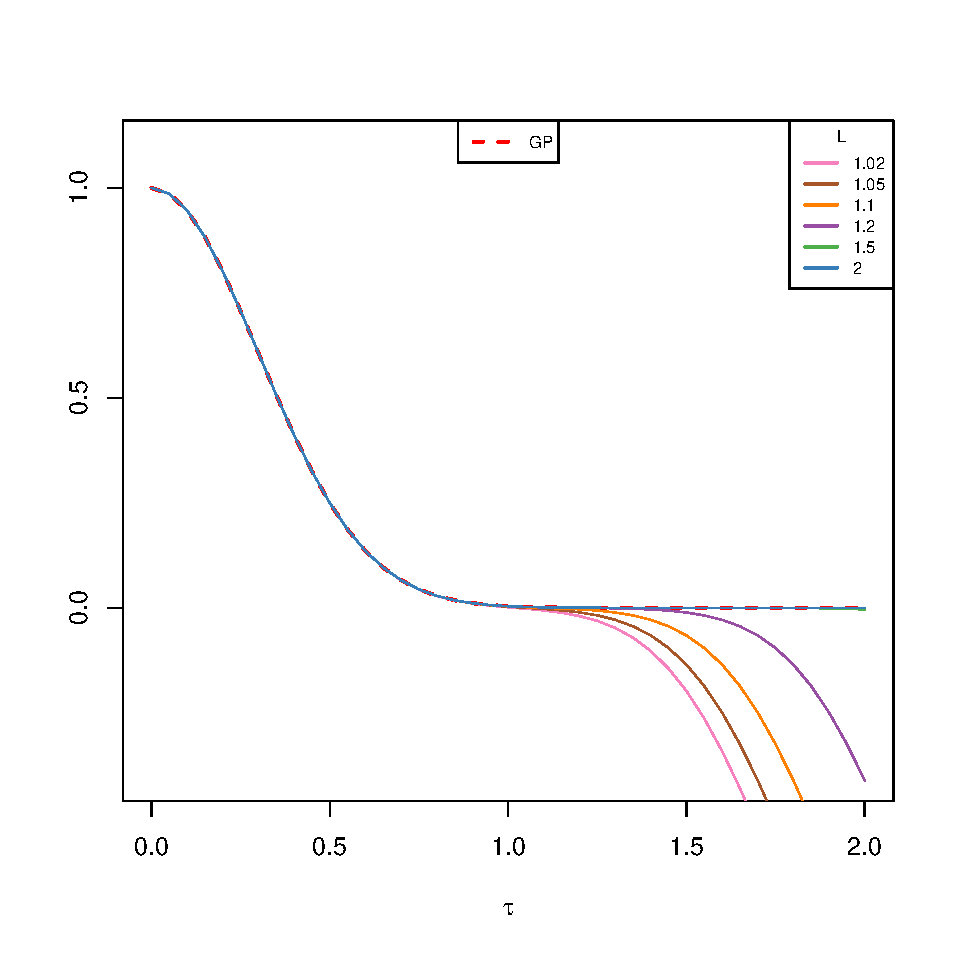
\includegraphics[scale=0.4]{fig2_Cov_L.pdf}}
\caption{(left) Posterior means for different different values of the box size $L$. (right) Covariance functions for different values of the box size $L$.}
  \label{fig2_Post_L}
\end{figure}

Therefore, the approximation to the covariance function depends on the number of basis functions $J$ used in the series expansion and the value for boundary condition or box size $L$. Additionally, there exit a relation among the number of basis functions, the box size and the lengthscale or roughness of the process on the performance of the approximation. Figure \ref{fig3_lscale_vs_J_vs_c_part1} collects how these three factors relate each other in order to achieve a good approximation to the covariance function of the regular GP using eq. (\ref{diff_covs}). On the X-axis of this plot is placed the lengthscale of the process normalized by the half-range of the data. The countour lines gather the box size which is also normalized by the half-range of the data, to which we refer as the boundary factor $c$, where $L=c \cdot \text{range}(x)/2$. And the Y-axis gathers the number of basis functions. Thus, this figure give us the minimum number of basis functions needed to achieve a good approximation in terms of satisfying eq. (\ref{diff_covs}), for a certain GP process with lengthscale $\ell$ and given a fixed boundary factor $c$. Alternatively, this figure could also be read as the maximum boundary factor $c$ that we should use given a number of basis functions, for certain GP process with certain lengthscale. And also this figure could also be read as the maximum roughness in a process that can be fitted properly given a number of basis functions and a box size. Finally, this figure also gives us the minimum value for the boundary factor $c$ which is suitable for certain roughness or number of basis functions. This figure basically collects the behaviour of the approximate GP model in function of the lengthscale, number of basis functions and boundary condition:

$\bullet$ As the lengthscale or smoothness of the process increase, the boundary factor and the number of basis functions needed for the approach decrease.

$\bullet$ There is a minimum boundary factor to achieve a good approach in function of the lengthscale (The contour lines have an end in function of the lengthscale).

$\bullet$ The lower boundary factor, the fewer basis functions, and the lower lengthscales suitable to be fitted. 

$\bullet$ This plot serves as a diagnosis tool in the sense that if the estimated lengthscale is lower than that minimun generated by the figure for the chosen number of basis functions and boundary factor means that we would need to increase the number of basis functions or decrease the boundary factor.

$\bullet$ On the other hand, if the lengthscale is bigger than that generated by the figure then it means that the fit should be good.

Figure \ref{fig3_lscale_vs_J_vs_c_part1} is useful for the user to know the suitable values for the number of basis functions $J$ and the boundary factor $c$ to approach a certain process characterized by its lengthscale. This Figure will allow us to optimize computations which depends on the number of basis functions. Starting from some guess of the lengthscale of the process and knowing the range of the input data which we are interested in, the user can do a few iterative adjustments to obtain an optimal fit. This figure also provides a diagnosis tool of the fit, in the sense that if the estimated lengthscale is lower than the minimum lengthscale able to fit with the actual number of basis functions and box size, indicates that the number of basis functions needs to be increased or the box size decreased. 

\begin{figure}[H]
\centering
\subfigure{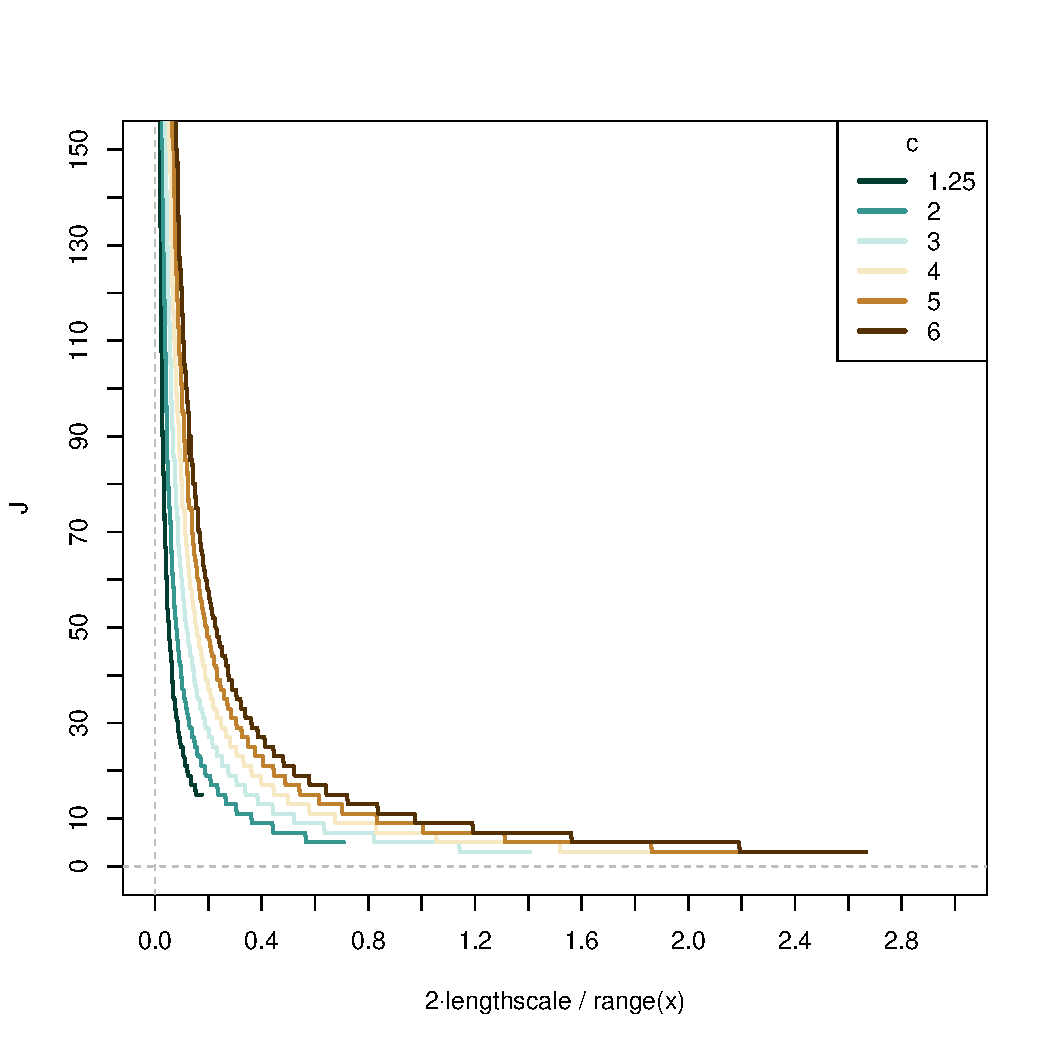
\includegraphics[scale=0.4]{fig3_lscale_vs_J_vs_c_part1.pdf}}
\subfigure{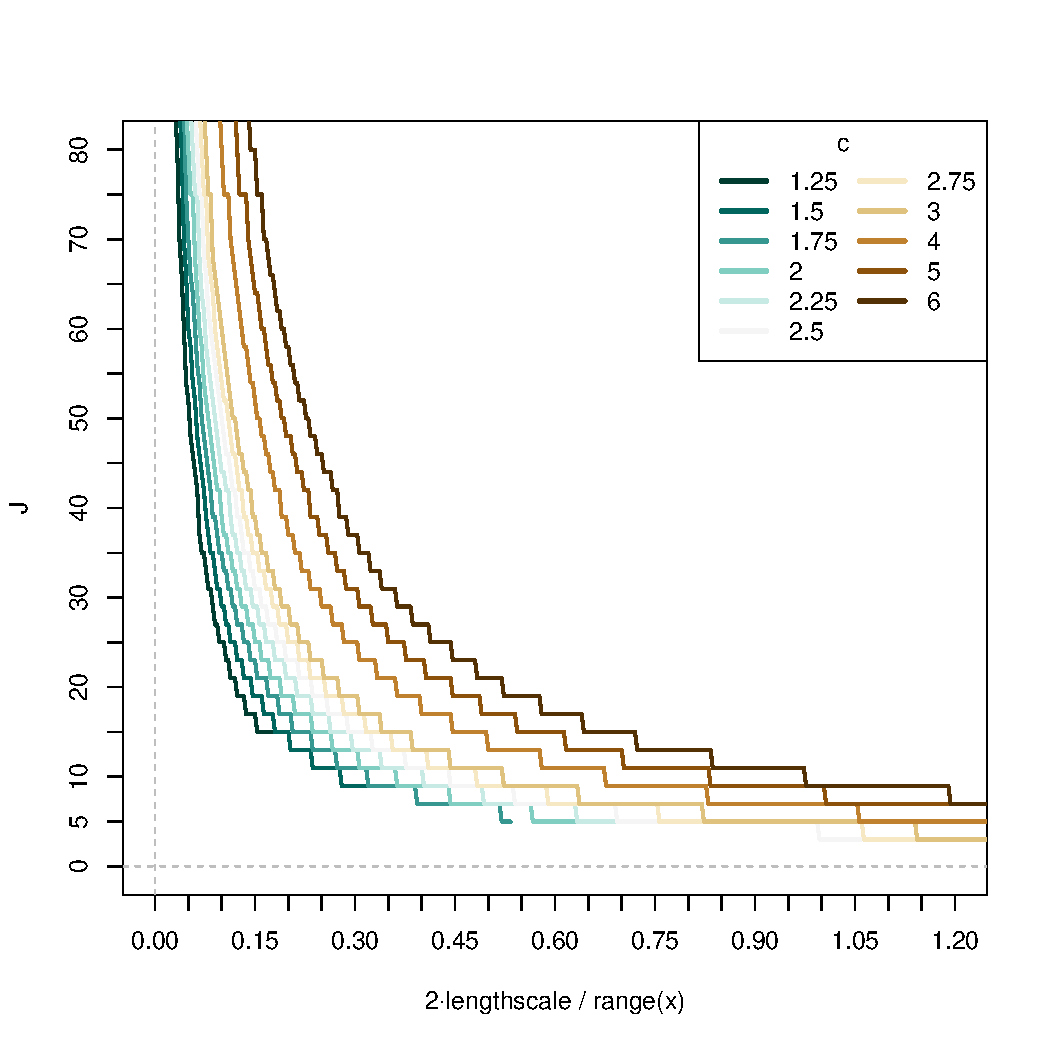
\includegraphics[scale=0.4]{fig3_lscale_vs_J_vs_c_part2.pdf}}
\caption{Relation between the minumum number of basis functions $J$, the lengthscale normalized by the half-range of the data ($\frac{\ell}{\frac{\text{range}(x)}{2}}$), and the boundary condition factor $c$ ($c = \frac{L}{\frac{\text{range}(x)}{2}}$).}
  \label{fig3_lscale_vs_J_vs_c_part1}
\end{figure}

The right-side plots in Figures \ref{fig1_Post_J} and \ref{fig2_Post_L} are computed using the lengthscale and magnitud values of the true GP prior. Now, we focus on the estimated lengthscale and magnitud parameters after fitting the model, either the regular GP model fit and the approximate GP model fit. Figure \ref{fig4_Post_&_Cov_part1} shows the posteriors distributions and the covariance functions of the approximate GP model and the regular GP model, obtained after fitting the data. Figure \ref{fig5_MSE_vs_J} shows the standarized root mean square error both models in function of the number of basis functions and the boundary factor. Figure \ref{fig6_lscale_vs_J} shows the evolution of the GP hyperparameters, lengthscale and magnitud, in function of the number of basis functions and boundary factor. Following Figure \ref{fig5_MSE_vs_J} it can be drawn that the optimal choice in terms of precision and computations would be 15 basis functions and a boundary factor between 1.5 and 2.5. The choice of 10 basis functions and a boundary factor of 1.5 could be accurate enough. This same conclusion can be roughly seen in the right-side plots in Figure \ref{image11_Posteriors_example-I}. This conclusions also agree with Figure \ref{fig3_lscale_vs_J_vs_c_part1} from which we can deduce that for a process with a normalized lengthscale of 0.3, 10 basis functions and a normalized box size (boundary factor) of 1.5 would be enough to get a good approximation following eq. (\ref{diff_covs}). 

From Figure \ref{fig5_MSE_vs_J} it can also be drawn the behaviour in terms of performance of the approximate GP model in function of the number of basis functions and the boundary factor. Two main behaviours can be deduced from Figure \ref{fig5_MSE_vs_J}, which can also be easily seen from Figure \ref{fig3_lscale_vs_J_vs_c_part1}:
\\ 
$\bullet$ as the boundary factor increases, more basis functions are needed,
\\
$\bullet$ as fewer basis functions are used, the boundary factor must decrease.  

Figure \ref{fig6_lscale_vs_J} shows the estimated lengthscale and magnitud parameter as function of the number of basis functions and the boundary factor. The same conclusion drawn before can be drawn form this figure where with 15 basis functions and a boundary factor of 1.5 the estimated lengthscale of the approximate GP model approach the estimeted lengthscale of the regular GP model. From this figure it can be drawn that exists a minumum value for the boundary factor under this never a good approach will be achieved. This conclusion also appears in Figure \ref{fig3_lscale_vs_J_vs_c_part1} the contour lines of the boundary factor have an end at certain lengthscales, which means that exist a minimum boundary factor depending on the lengthscale of the process. 

\begin{figure}[H]
\centering
\subfigure{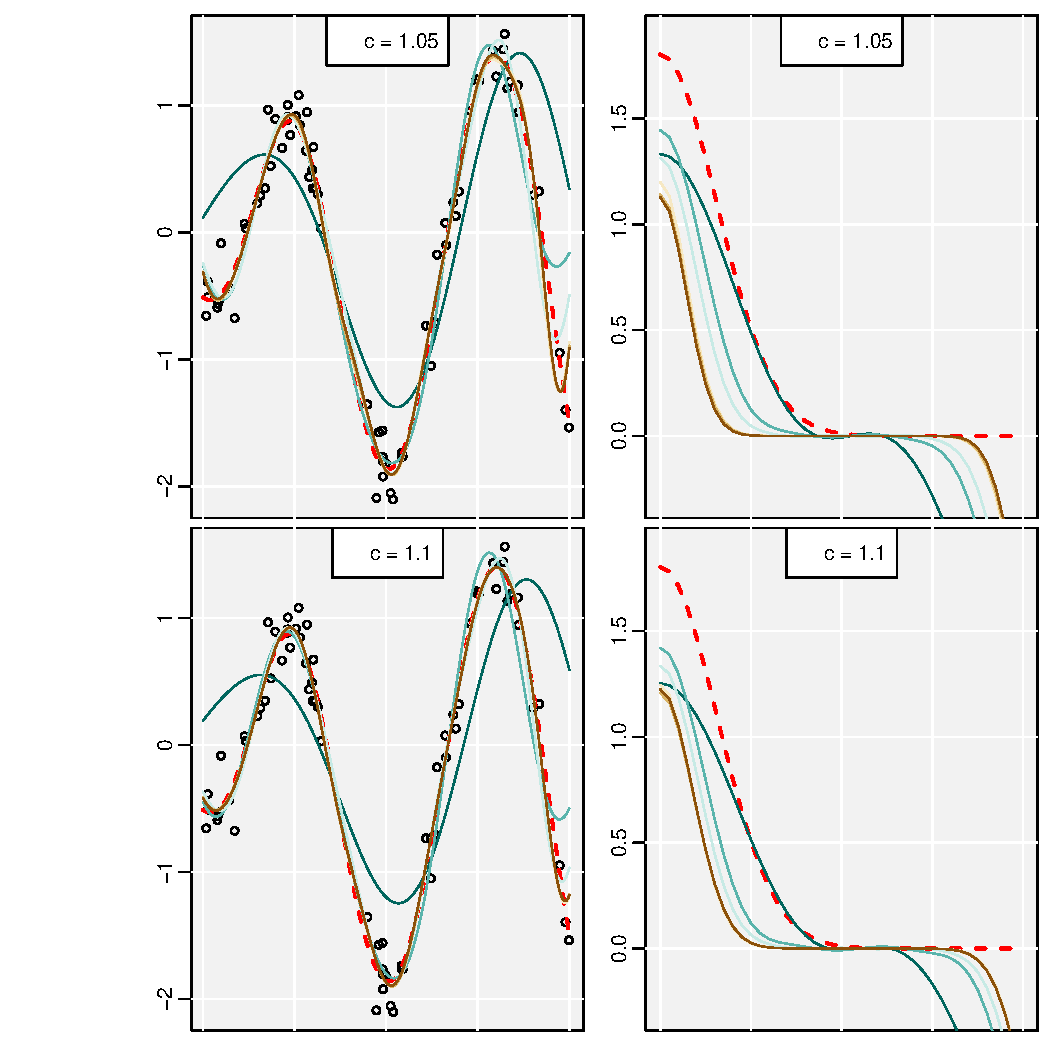
\includegraphics[scale=0.6]{fig4_Post_&_Cov_part1.pdf}}
\subfigure{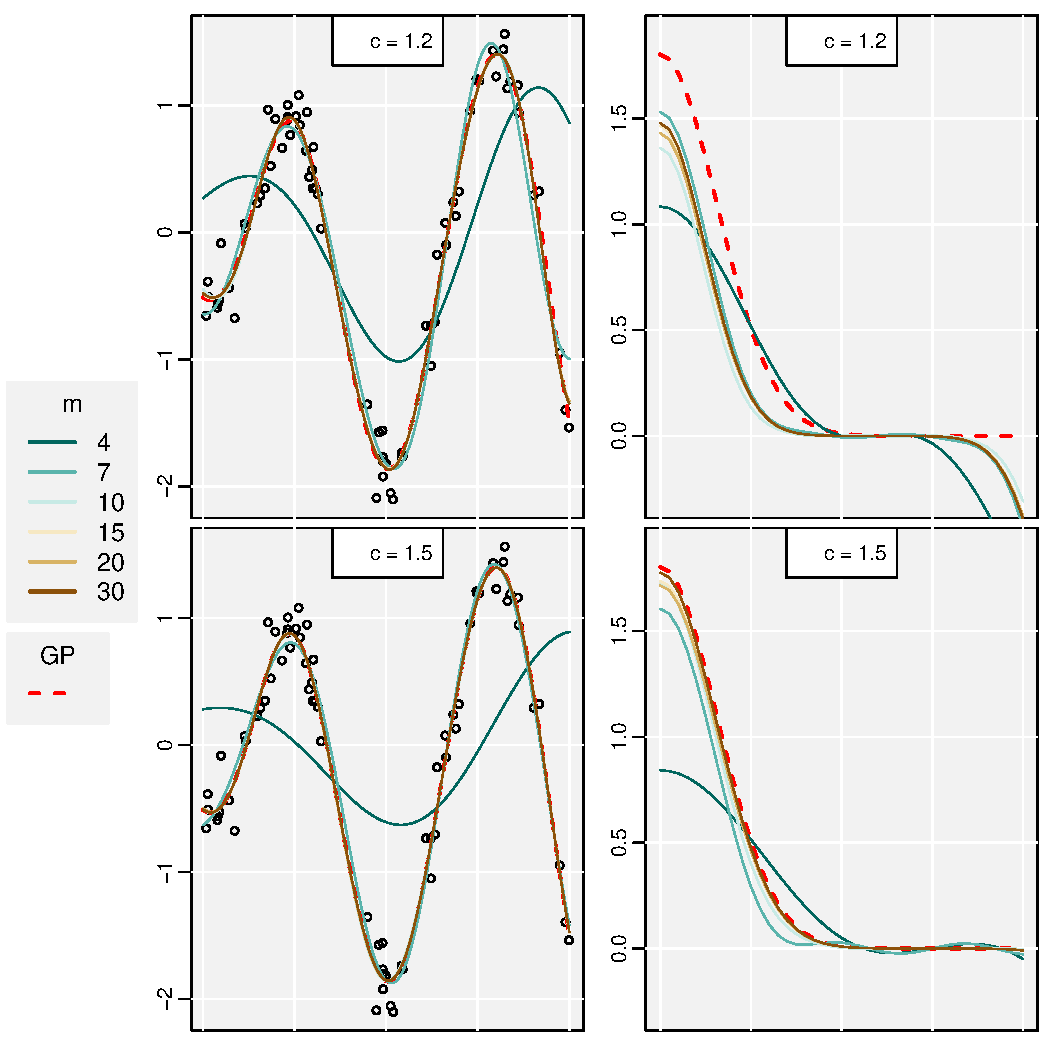
\includegraphics[scale=0.6]{fig4_Post_&_Cov_part2.pdf}}
\caption{Posterior distributions and covariance functions of the proposed approximate GP models and the exact GP model in function of the number of basis functions $J$ and the boundary factor $c$.}
  \label{fig4_Post_&_Cov_part1}
\end{figure}

\begin{figure}[H]
\centering
\subfigure{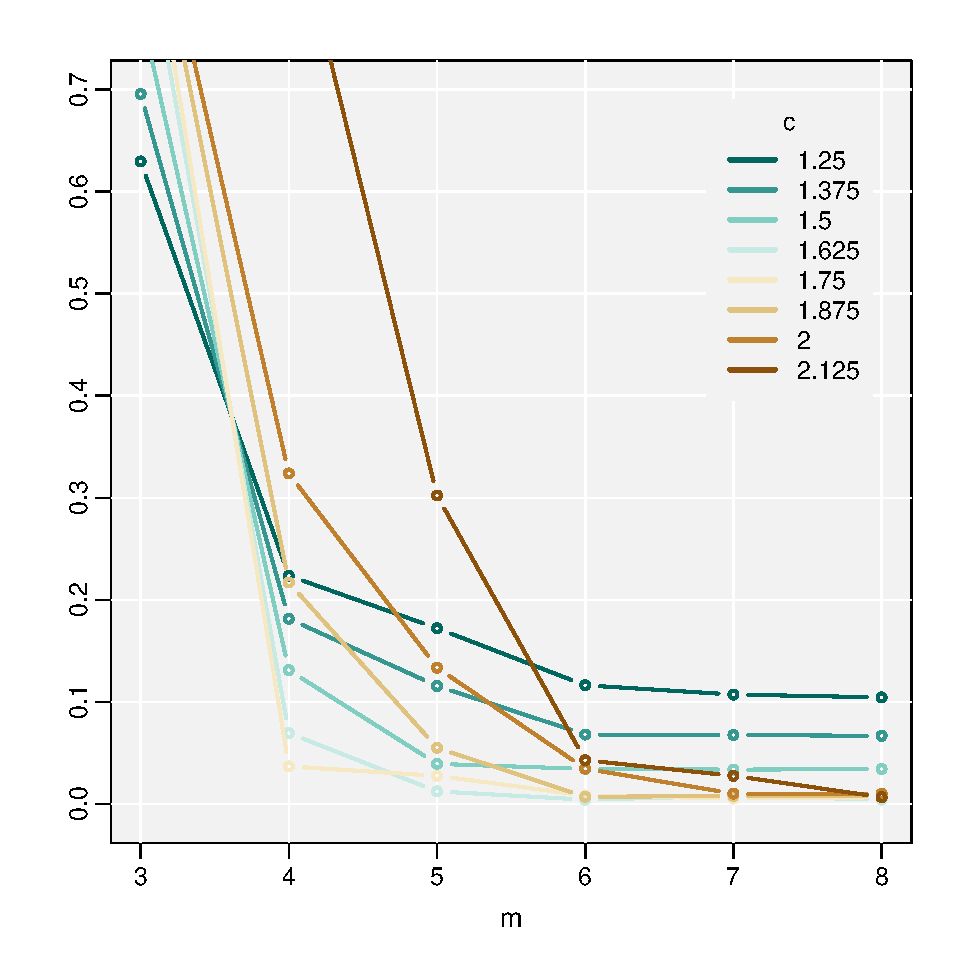
\includegraphics[scale=0.4]{fig5_MSE_vs_J.pdf}}
\subfigure{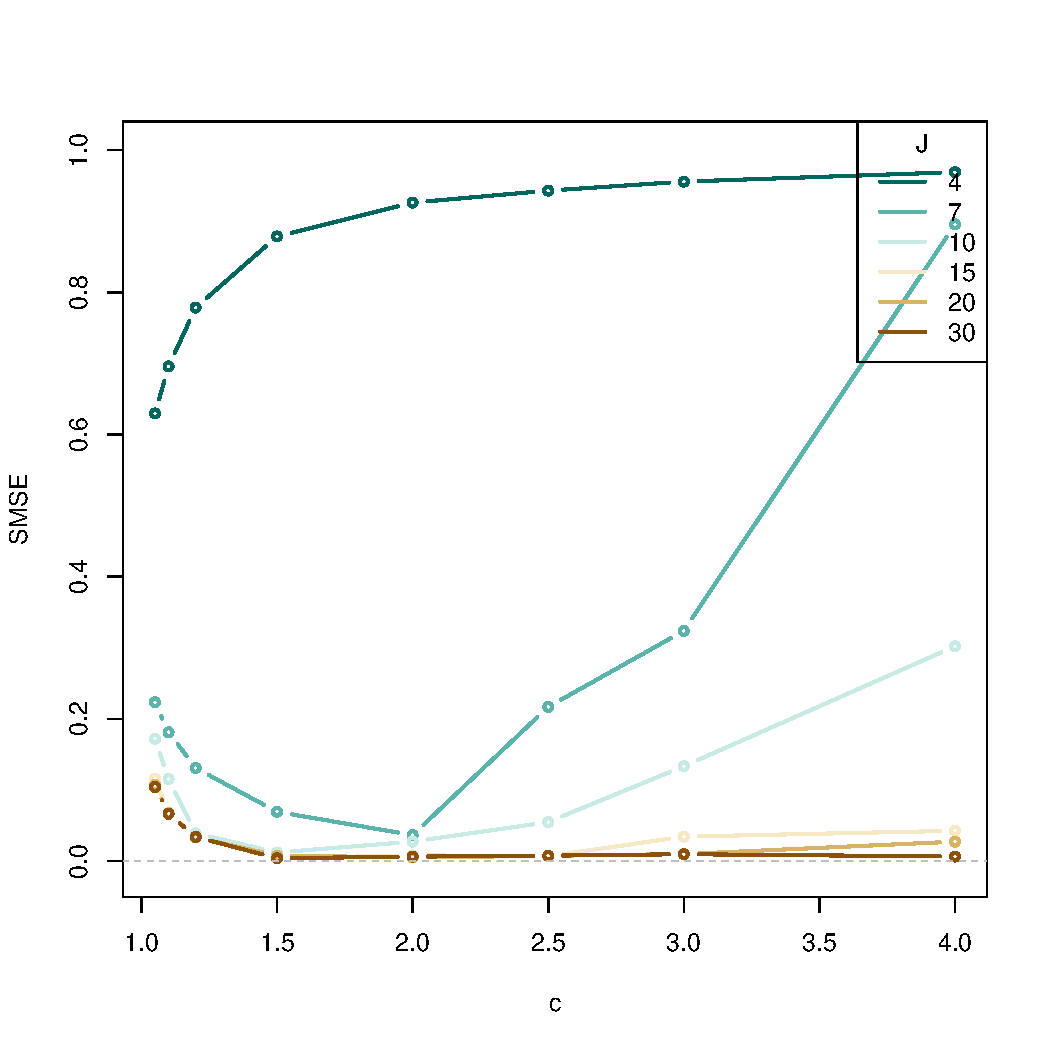
\includegraphics[scale=0.4]{fig5_MSE_vs_c.pdf}}
\caption{Standarized root mean square error (SRMSE) of the proposed approximate GP models and the exact GP model. (left) SRMSE against the number of basis functions $J$ for different values of the boundary factor $c$. (right) SRMSE against the boundary factor $c$ for different values of the number of basis functions $J$. }
  \label{fig5_MSE_vs_J}
\end{figure}

\begin{figure}[H]
\centering
\subfigure{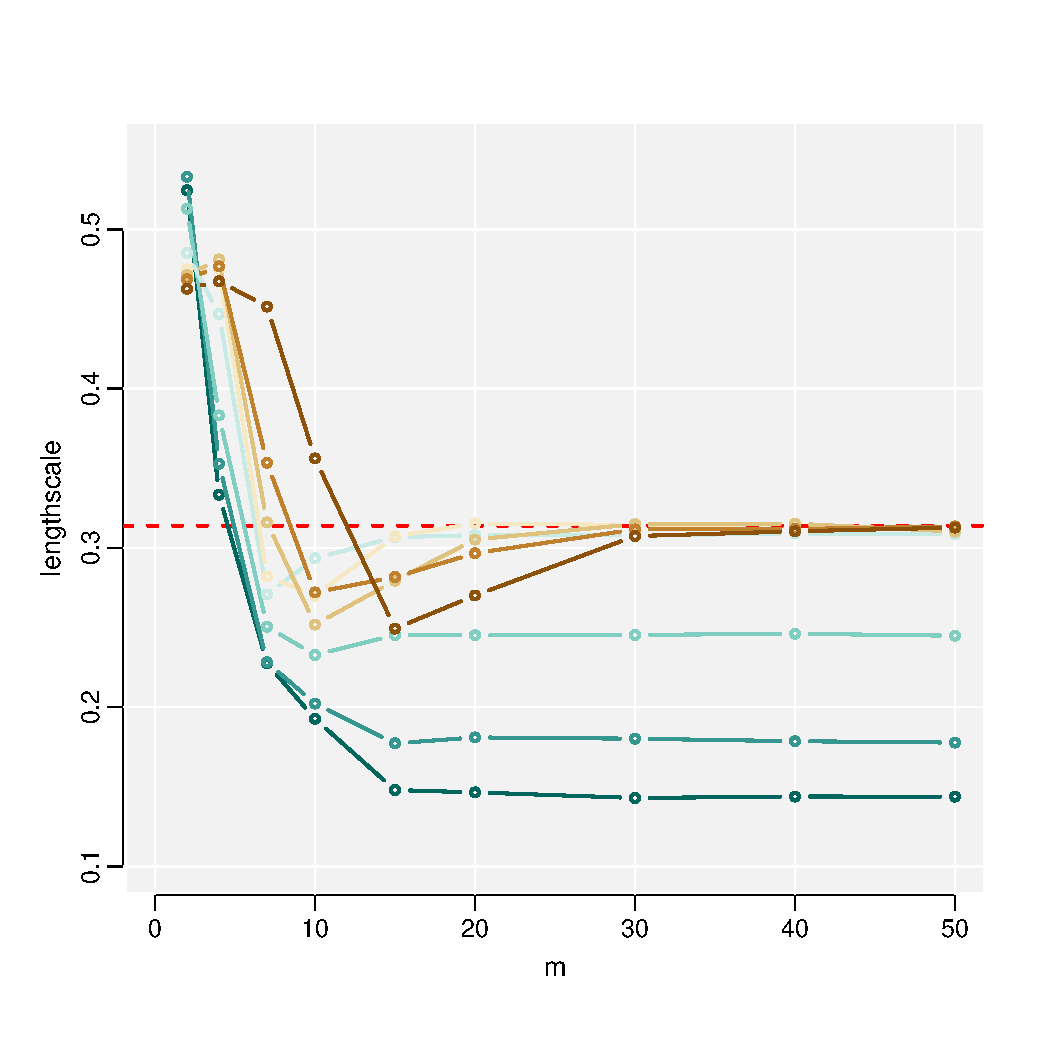
\includegraphics[scale=0.4]{fig6_lscale_vs_J.pdf}}
\subfigure{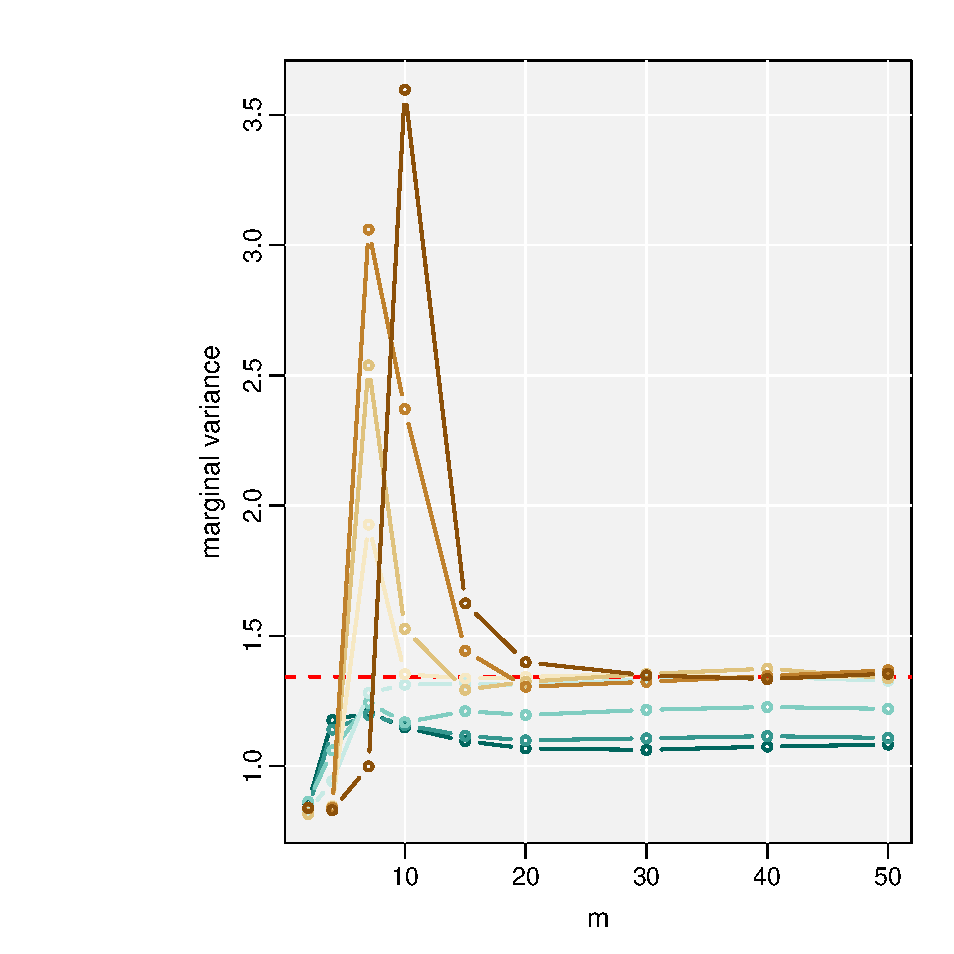
\includegraphics[scale=0.4]{fig6_magnitud_vs_J.pdf}}
\caption{(left) Estimated lengthscales against the number of basis functions $J$ for different values of the boundary factor $c$. (right) Estimated GP magnitud the number of basis functions $J$ for different values of the boundary factor $c$. }
  \label{fig6_lscale_vs_J}
\end{figure}

\subsection{Comparative between true lengthscales and estimated lengthscales}

In this section we fit the regular GP model and the approximate GP model on different datasets drawn from GP prior models with a squared exponential covariance function with different lengthscales. The approximate GP model is fitted using different number of basis functions.

\begin{figure}[H]
\centering
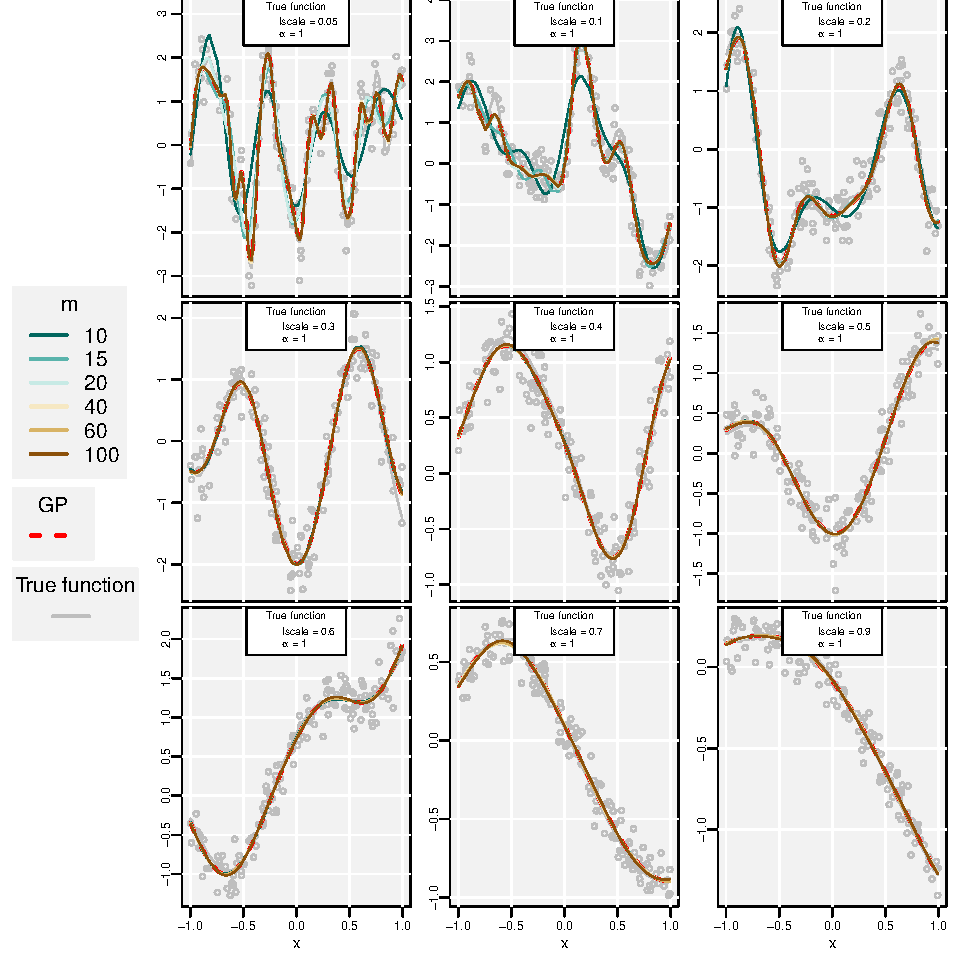
\includegraphics[scale=0.4]{fig7_varing_lscale.pdf}
\caption{Posterior means of the exact and approximate GP models fitted over different datasets with different lengthscales.}
  \label{fig7_varing_lscale}
\end{figure}

Figure \ref{fig8_Tlscale_vs_Elscale} compares the true lengthscales to the estimated lengthscales for the exact GP and the approximate GP. The black line defines the minimun lengthscale that the approximate GP model can fit for each case.

\begin{figure}[H]
\centering
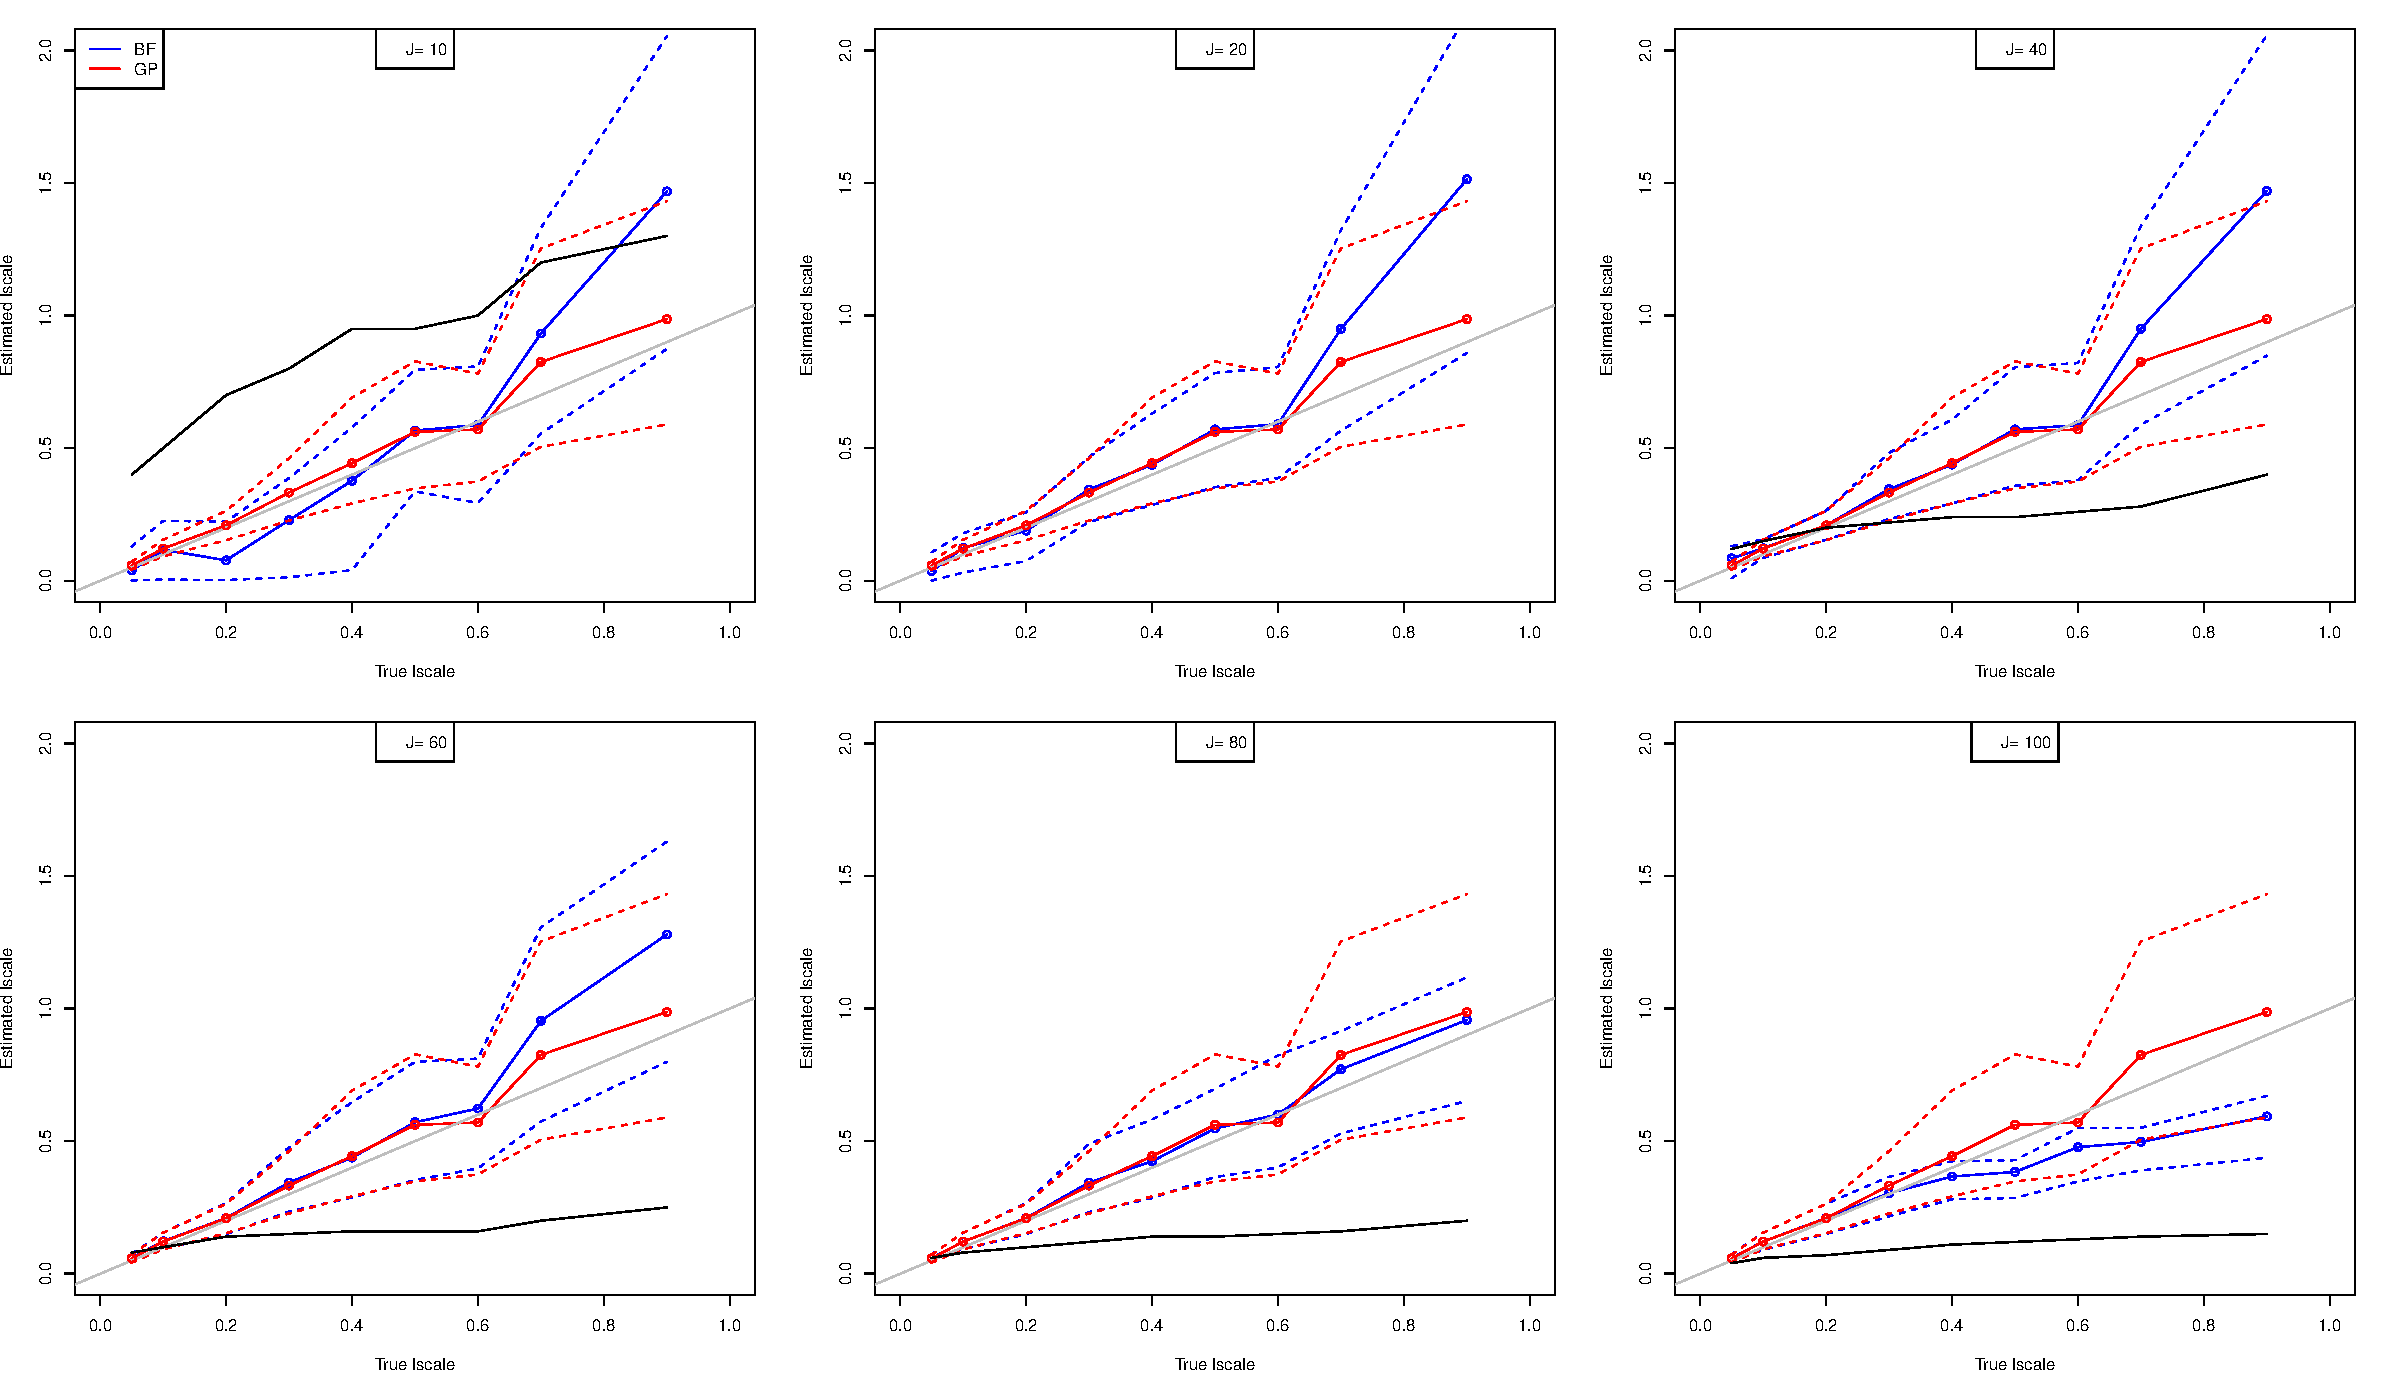
\includegraphics[scale=0.4]{fig8_Tlscale_vs_Elscale.pdf}
\caption{True lengthscales versus estimated lscales of the different realizations of datasets using different number of basis functions. }
  \label{fig8_Tlscale_vs_Elscale}
\end{figure}


\vspace{3mm}
\section{Univariate illustrative examples}\label{sec:gp_examples1D}


\subsection{Simulated data}

A simulated one-dimensional dataset, with 250 data points drawn from a Gaussian process prior with a Matern covariance function with 3/2 degrees of freedom. The hyperparameters of this GP prior with a Matern kernel, marginal variance and lengthscale are set to 1 and 0.15, respectively. The additive Gaussian noise to the GP model is set to 0.2. We compare the modelling performance over this simulated process of our proposed approach with the performance of a regular GP and a Splines-based model. For our basis function approach we use $J=80$ basis functions and a boundary factor $c=1.2$. For the Splines-based model we use 80 knots or basis in the model.

Figure \ref{fig9_Posteriors_exI} shows the posteriors distributions of the proposed model and the regular GP model, fitted over the simulated dataset. Posteriors distributions of the proposed approximation GP model, of the exact GP model, and the Splines model are plotted jointly with the true GP prior from the data were drawn. The right and left extremes of the simulated data correspond to out-of-sample data or test data which have not been taking part of training the models. Over this test data we can evaluate the predictive performance of every method.  

\begin{figure}[H]
\centering
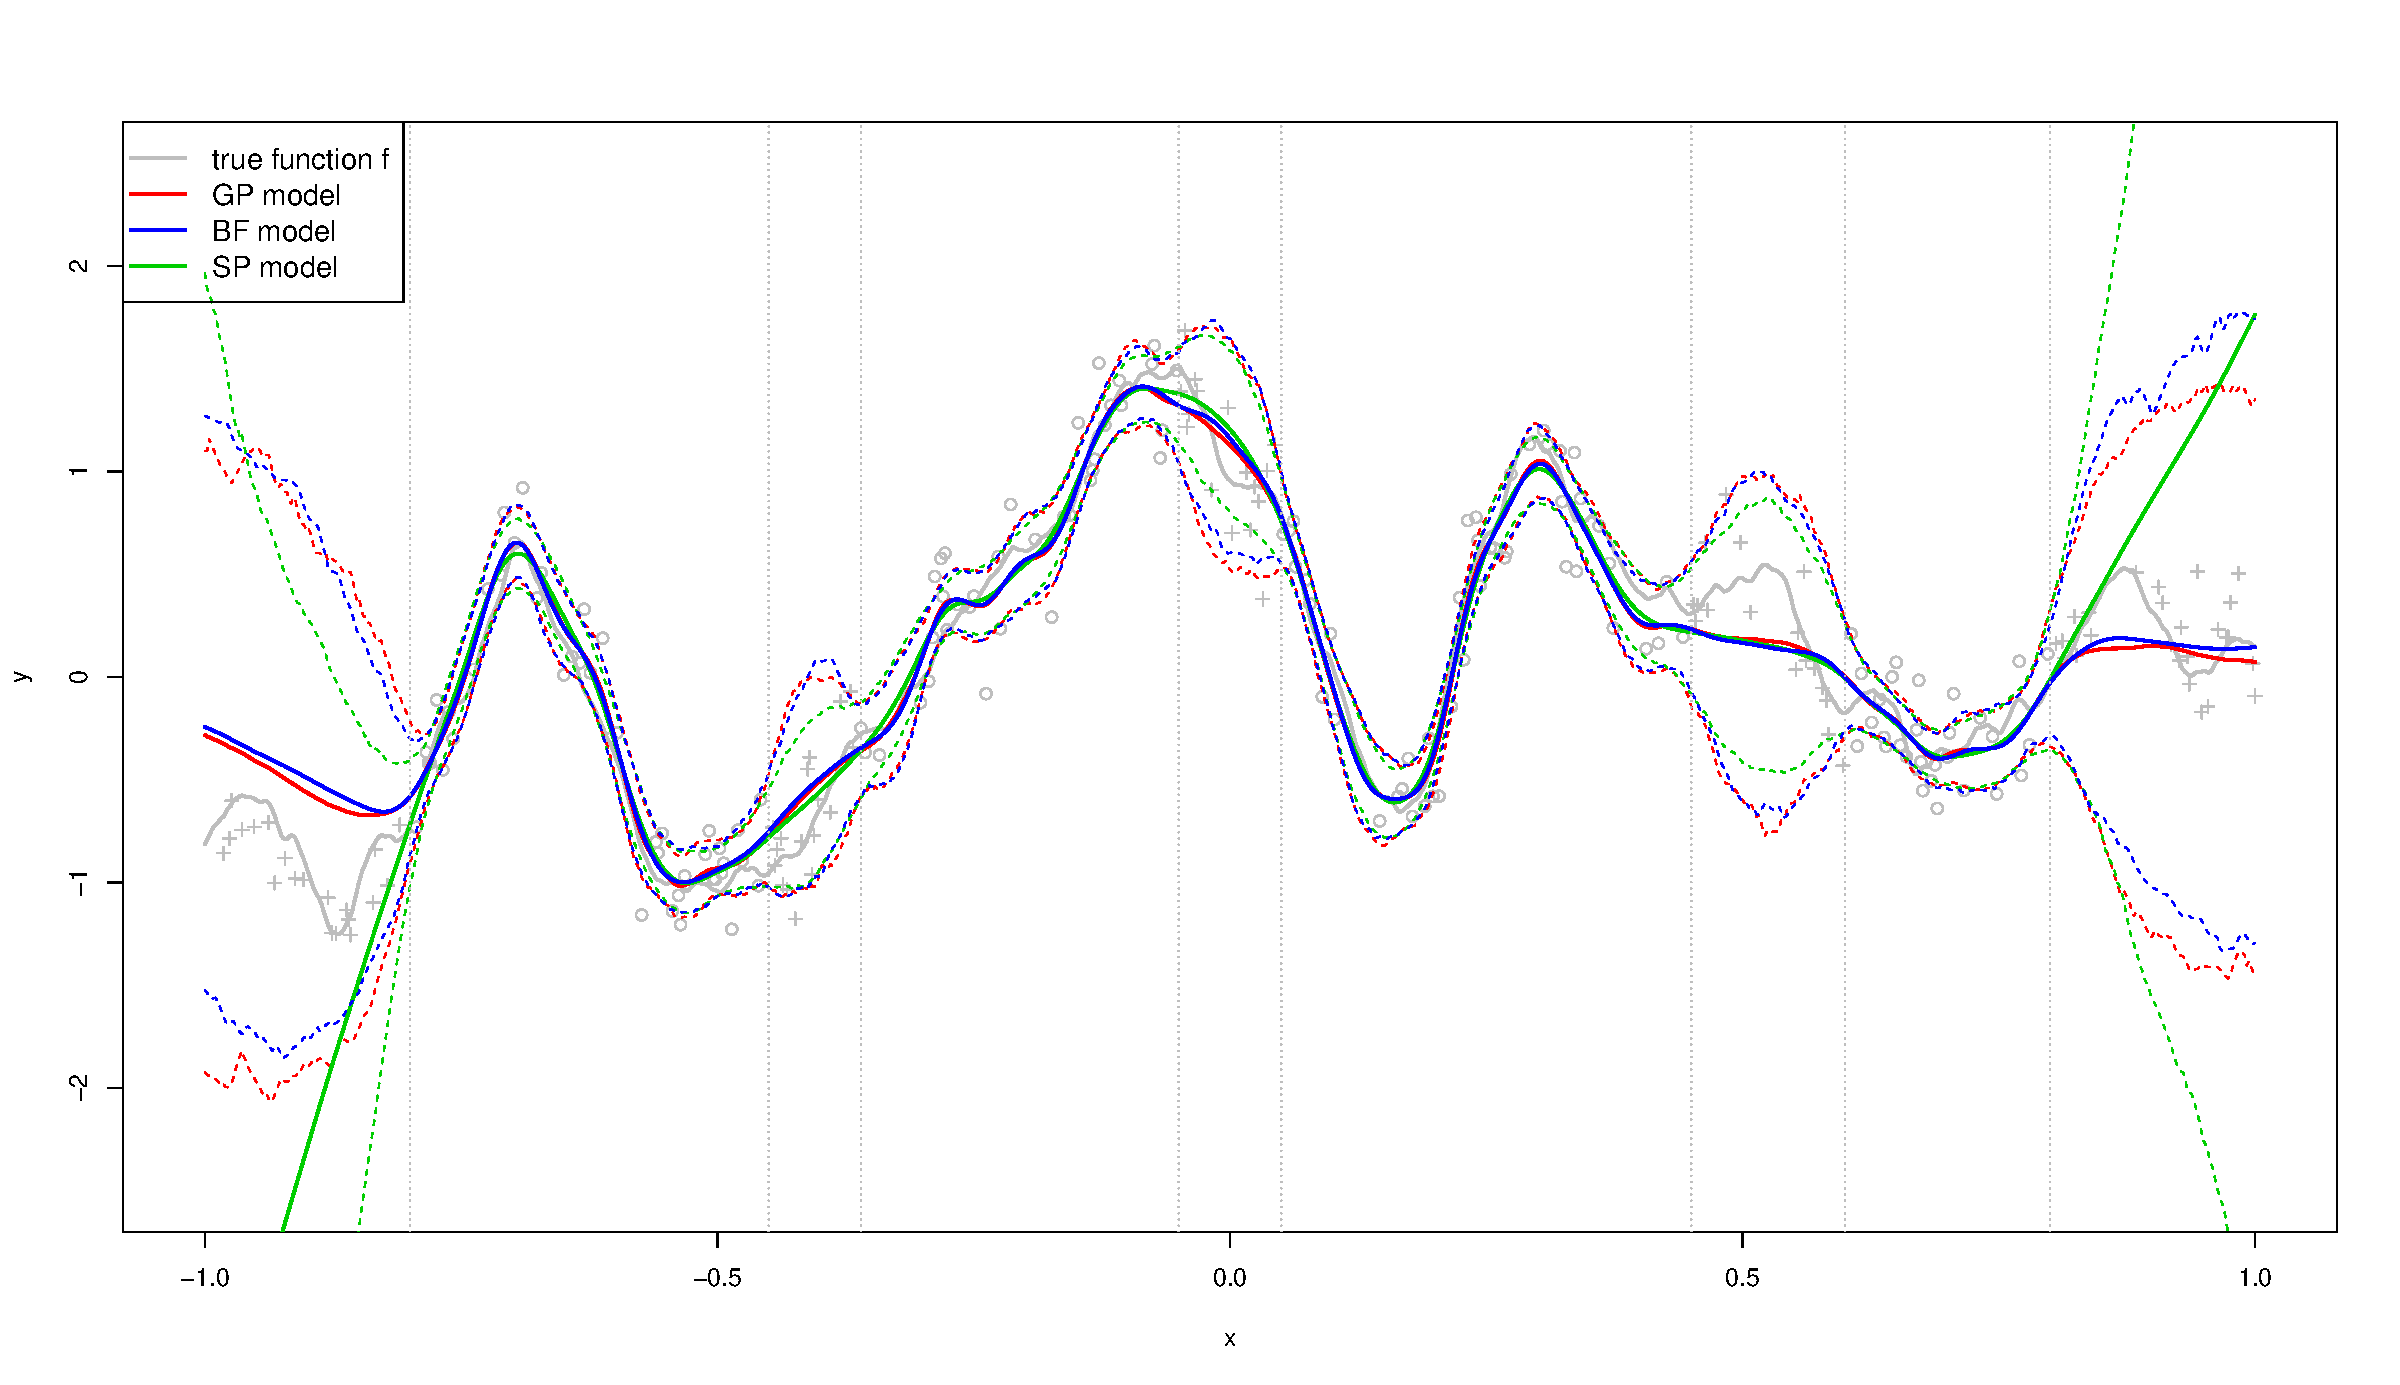
\includegraphics[scale=0.35]{fig9_Posteriors_exI.pdf}
\caption{Posterior distributions of the proposed approximated GP model, the exact GP model, and the Splines model.}
  \label{fig9_Posteriors_exI}
\end{figure}

For assessing the performance of different methods we use the standardized mean squared error (SMSE) over the true function for interpolation and extrapolation data. 

\begin{figure}[H]
\centering
\subfigure{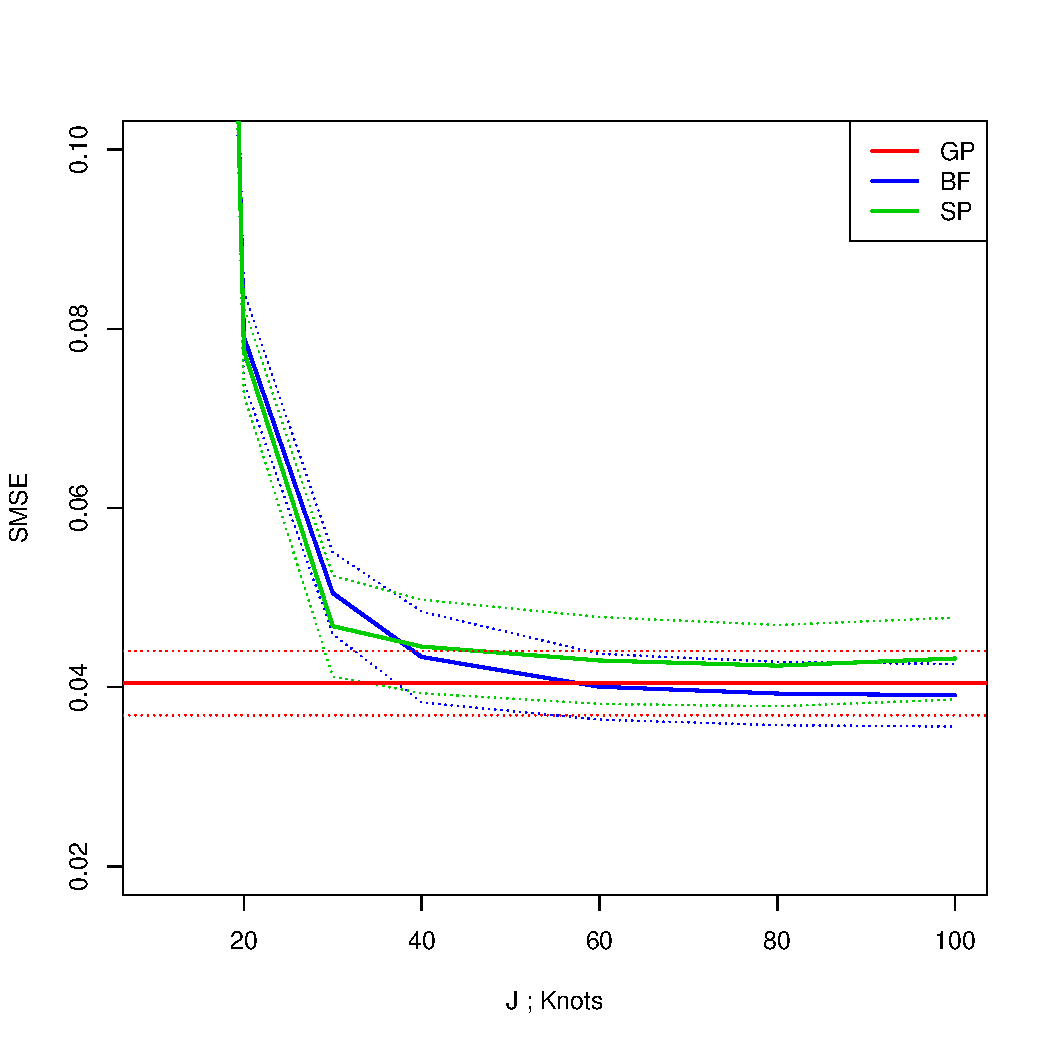
\includegraphics[scale=0.350]{fig10_MSE_exI_inter.pdf}}
\subfigure{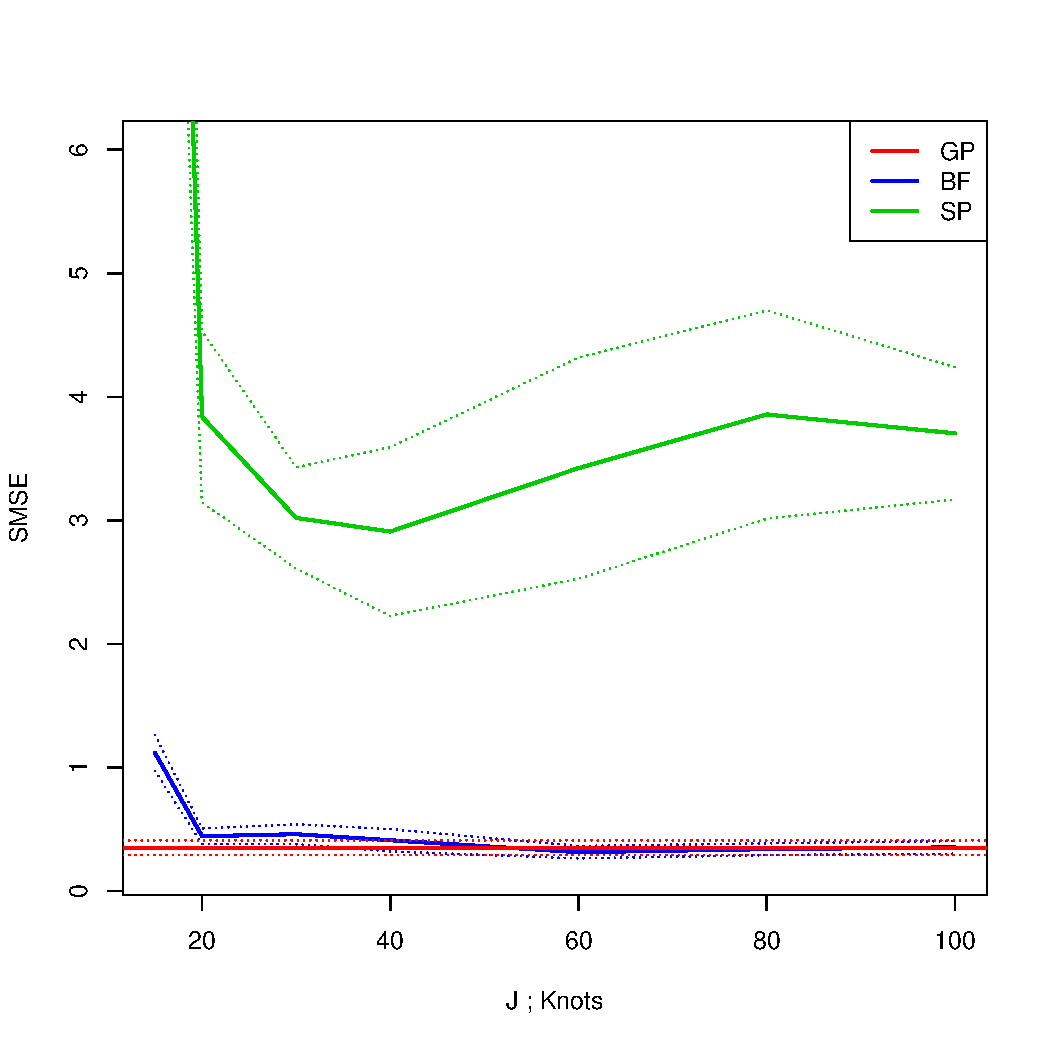
\includegraphics[scale=0.350]{fig10_MSE_exI_extra.pdf}}
\caption{Standarized mean square error (SMSE) of the different methods againts the true function. (left) SMSE for interpolation. (right) SMSE for extrapolation}
  \label{fig10_MSE_exI_inter}
\end{figure}

\subsection{Case I: Gay data}\label{sec:bf_caseII}
\subsection{Case II: Birthday data}\label{sec:bf_caseIII}

\vspace{3mm}
\section{Multivariate illustrative examples}\label{sec:gp_examplesMulti}
\subsection{Simulated data}\label{sec:bf_toyexampleMulti}
\subsection{Case III: Diabetes data}\label{sec:bf_caseIV}
\subsection{Case IV: Leukemia data}\label{sec:bf_caseV}
\subsection{Case V: Land use spatio-temporal classification task}\label{sec:bf_caseVII}

\vspace{3mm}
\appendix

\section{Related work}

The GP prior entails an $O(n^3)$ complexity that is computationally intractable for many practical problems, and this problem especially becomes severe when we want to conduct inference using sampling methods. To overcome this scaling problem several schemes have been proposed. One approach is to partition the data set into separate groups \citep{snelson2007local, urtasun2008sparse} and performing local inference in each partition. Other global approach is to build a low-rank approximation to the covariance matrix of the complete data based around 'inducing variables' \citep{quinonero2005unifying,bui2017unifying}. Other global approach make use of basis functions to approximate the covariance function. In \cite{snelson2007local} the authors conduct an approach that combines the idea of local and global approaches.

The literature contains many parametric models that approximate Gaussian process behaviours; for example \cite{bui2014tree} included  tree-structures in the approximation for extra scalability, and \cite{moore2015gaussian} combined local Gaussian
processes with Gaussian random fields.

\subsection{Inducing points methods}

The approach based on inducing points employs a small set of pseudo data points to summarise the actual data. The storage requirements are reduced to $O(nm)$ and complexity to $O(nm^2)$, where $m < n$. Some of these methods have been reviewed in \cite{rasmussen2006gaussian}, and \cite{quinonero2005unifying} provide a unifying view of these methods based on approximate generative methods. From a spectral point of view, several of these methods (e.g., SOR, DTC, VAR, FIC) can be interpreted as modifications to the so-called Nystr\"om method (see \cite{arthur1979baker} and \cite{williams2001using}), a scheme for approximating the eigenspectrum. These methods are basically based on choosing a set of $m$ inducing inputs $x_u$ and scaling the corresponding eigendecomposition of their corresponding covariance matrix $K_{u,u}$ to match that of the actual covariance. 

This scheme was originally introduced to the GP context by \cite{williams2001using}. As discussed by \cite{quinonero2005unifying}, the Nystr\"om method by \cite{williams2001using} does not correspond to a well-formed probabilistic model. However, several methods modifying the inducing point approach are widely used. The Subset of Regressors (SoR) \citep{smola2001sparse} method uses the Nystr\"om approximation scheme and a finite linear-in-the-parameters model for approximating the whole (training and test) covariance function, whereas the sparse Nystr\"om method \citep{williams2001using} only replaces the training data covariance matrix. The SoR method is based on a degenarete prior which produces unresoanble predictive uncertainties, which is a general problem of linear models (for more details see \cite{rasmussen2006gaussian}). 

The Deterministic Training Conditional (DTC) method \citep{ro2001sparse,seeger2003fast}) retains the true covariance for the training data, but uses the approximate cross-covariances between training and test data, which reverse the problem of nonsensical predictive uncertainties. However, since the covariances for training and test cases are computed differently, this method results not to actually be a Gaussian process. This method was presented as Projected Latent Variables (PLV) in \cite{seeger2003fast} and Projected Process Approximation (PPA) in \cite{rasmussen2006gaussian}. 

The Variational Approximation (VAR) \citep{titsias2009variational} suggests a variational approach which provides an objective function for optimizing the selection of inducing points. This basically modifies the DTC method by an additional trace term in the likelihood that comes from the variational bound.  \cite{hensman2013gaussian} extended this idea by introducing additional variational parameters to enable stochastic variational inference \citep{hoffman2013stochastic}, achieving a more computationally scalable bound which allows GPs to be fitted to millions of data.

The Fully Independent (Training) Conditional (FIC) \citep{quinonero2005unifying} method originally introduced as Sparse Pseudo-Input GP by \cite{snelson2006sparse} is also based on the Nystr\"om approximation, where they allow the pseudo-point input locations to be optimised by maximising the new model's marginal likelihood whose covariance is parameterized by the locations of an active set not constrained to be a subset of the training and test data.

More recently Bui et. al (2017) revisit the inducing points-based sparse approximation methods, in which all the necessary approximation is performed at inference time, rather than at the modelling time. The new framework is built on standard methods for approximate inference (variational-free-inference, EP and Power EP methods). 

In practice, the inducing points-based sparse approximation methods works reasonable well in cases where the field is relatively smooth. \cite{vanhatalo2010approximate}
propose the use of compactly supported covariance function in conjunction with sparse approximations to model both short and long range correlations.

\cite{wilson2015kernel} introduce a new unifying framework for inducing point methods, called structured kernel interpolation (SKI). This framework improves the scalability and accuracy of fast kernel approximations through kernel interpolation, and naturally combines the advantages of inducing point and structure exploiting for scalability (such as Kronecker \citep{saatcci2012scalable} or Toeplitz \citep{cunningham2008fast}) approaches.

The number of inducing points or their locations are crucial in order to capture the correlation structure. For a discussion on the effects of the inducing points, see \cite{vanhatalo2010approximate}. This behavior applies to all the methods from the Nystr\''om family.

This kind of 'projected process' approximation has also been discussed by e.g. \cite{banerjee2008gaussian}.


\subsection{Basis function methods}

The spectral analysis and series expansions of Gaussian processes has a long history. A classical result (see, e.g, \cite{loeve1977probability,trees1968detection,adler1981geometry,cramer2013stationary}, and references therein) is that the covariance function can be approximated with a finite truncation of Mercer series and the approximation is guaranteed to converge to the exact covariance function when the number of terms is increased. 

Another related classical connection is to the works in the relationship of spline interpolation and Gaussian process priors \citep{wahba1978improper,kimeldorf1970correspondence,wahba1990spline}. In particular, it is well-known (see, e.g., \cite{wahba1990spline}) that spline smoothing can be seen as Gaussian process regression with a specific choice of covariance function. The relationship of the spline regularization with Laplace operators then leads to series expansion representations that are closely related to the approximations considered here. 

Random Fourier Features \citep{rahimi2008random,rahimi2009weighted} is a method for approximating kernels. The approximate kernel has a finite basis function expansion.


The Sparse Spectrum GP is based on a sparse approximation to the frequency domain representation of a GP \citep{lazaro2010sparse,quia2010sparse}, where the spectral representation of the covariance function is used. This model is a stationary sparse GP that can approximate any desired stationary full GP. However, as argued by the authors, this option does not converge to the full GP and can suffer from overfitting to the training data. \citep{gal2015improving} sought to improve the model by integrating out, rather than optimizing the frequencies. Gal and Turner derived a variational approximation that made use of a tractable integral over the frequency space. The result is an  algorithm that suffers less overfitting than the Sparse Spectrum GP, yet remains flexible.

While Sparse Spectrum GP is based on a sparse spectrum, the reduced-rank method proposed in this paper aims to make the spectrum as ‘full’ as possible at a given rank.

Recently \citep{hensman2017variational} presented a variational Fourier feature approximation for Gaussian processes that was derived for the Mat´ern class of kernels, where the approximation structure is set up by a low-rank plus diagonal structure. They combine the variational methodology with Fourier based approximations.

In spatial statistics similar approaches are called low-rank models \citep{diggle2007springer}. The low rank models assume that the Gaussian field is a linear combination of $m$ basis functions. The type of an approximation depends on the basis functions used. Familiar examples include spectral representation \citep{diggle2007springer,paciorek2007computational,paciorek2007bayesian} and splines \citep{wood2003thin}. 

Recent Splines models can reproduce the Matern family of covariance functions, however our approach can reproduce basically all of the stationary covariance functions.


\section{Contributions of the method}

This work is based on the novel method developed by \cite{solin2018hilbert} for reduced-rank approximations of GP models. This method is based on interpreting the covariance function as the kernel of a pseudo-differential operator and approximating it using Hilbert space methods. This results in a reduced-rank approximation for the covariance function. This method has some nice features:

\vspace{2mm}
$\bullet$ It has an attractive computational cost as this basically turns the regular GP model into a lineal model.

\vspace{2mm}
$\bullet$ In a fully Bayesian inference framework using sampling methods, the proposed approximate GP model has a computational complexity of $O(nm+m)$ in every step of the HMC method. In addition, the computation of the automatic differentation to compute the gradients in this linear model scales $O(n)$?, an operation that must be computed in every step of the HMC method.

\vspace{2mm}
$\bullet$ Using maximizing marginal likelihood methods, the proposed model has a overall complexity of $O(nm^2)$. After this, evaluating the marginal likelihood and marginal likelihood gradients is an $O(m^3)$ operation in every step of the optimizer. (Arno's paper, pag. 7)

\vspace{2mm}
$\bullet$ The parameter posterior distribution in this approximate GP model is $m$-dimensional ($m<<n$) which helps the use of GP priors as latent functions. especially when sampling methods for inference are used. GP prior as latent functions is needed in generalized models.

In regular GPs and other approximate GP models and Splines models these features do not have so nice properties:

\vspace{2mm}
$\bullet$ In a regular GPs, the main computational complexity comes from the inversion of the covariance matrix which is in general a $O(n^3)$ operation. This operation has to be computed at every step of the HMC or optimizer.

\vspace{2mm}
$\bullet$ In regular GPs, the parameter posterior distributions is $N$-dimensional. It is known that when $N$ is of medium or large size there is high correlation between the $N$-dimensional latent function and the hyperparameters of the GP prior.

\vspace{2mm}
$\bullet$ In conventional sparse GP approximations, although the rank of the GP is reduced considerably to the number of inducing points, this still needs to do the autodiff and covariane matrix inversion.

\vspace{2mm}
$\bullet$ The Splines models are also a sort of basis functions expansion model, then the computational demands are similar to that in this approach. However in Splines models the lengthscale hyperparameter tend to be fixed and then the fit is covered by the magnitud parameter. In that sense, Splines models tend to loose the useful interpretation of the lengthscale parameter.



\section{Contributions of our work}

As said above the proposed method was already developed by \cite{solin2018hilbert} where they fully develop, describe and generalize the methodology. Though, they do not put much effort in describing and analyzing the relation among the key factors of the box size (or boundary condition), the number of basis functions, and the smoothness or roughness of the function. The performance and accuracy of the method are directly related with the number of basis functions and the box size. At the same time, successful values for these two factors depend on the smoothness or roughness of the process to be modeled. The time of computation is mainly dependent on the number of basis functions. Our main contributions to this recently developed methodology for low-rank GP model by \cite{solin2018hilbert} goes around these aspects.

\vspace{2mm}
$\bullet$ Firstly, clear summarized formulae of the method for the univariate and multivariate cases is presented. 

\vspace{2mm}
$\bullet$ We investigate the relations going on among these factors, the number of basis functions, the box size, and the lengthsccale of the functions.

\vspace{2mm}
$\bullet$ We make recomendations for the values of these factors based on the recognized relations among them. We provide useful graphs of these relations that will help the users to improve performance and save time of computation.

\vspace{2mm}
$\bullet$ We also diagnose if the chosen values for the number of basis functions and the box size are adequate to fit to the actual data.

\vspace{2mm}
$\bullet$ We describe the generalization of the method to the multidimensional case.

\vspace{2mm}
$\bullet$ We implement the approach in a fully probabilistic framework and for the Stan programming probabilistic software.

\vspace{2mm}
$\bullet$ We show several illustrative examples, simulate and real datasets, of the performance of the model, and accompanied by their Stan codes.

 
%\vspace{3mm}
%A summary of the formulae of the method for the univariate and multivariate cases is presented. The number of basis functions used in the approach and the value for the boundary condition of the model are two factors of main importance in practical applications. The number of basis functions is directly related to the accuracy of the approximation but also to the computation demands. Also exist a relation among the number of basis functions, the specified values for the boundary condition, and the performance of the approach.  Finally, the approach is applied in several illustrative study cases and accompanied by their Stan codes.

\section{Spectral densities of stationary covariance functions}

The covariance function of a stationary process, that is function of $\boldsymbol{\tau}=\mathbf{x-x'}$ can be represented as the Fourier transform of a positive finite measure ($Bochner's theorem$). 

\vspace{0.2cm}
\textit{(Bochner’s theorem) A complex-valued function $k$ on ${\rm I\!R}^D$ is the covariance function of a weakly stationary mean square continuous complex valued random process on ${\rm I\!R}^D$ if and only if it can be represented as}
%
\begin{equation}
k(\boldsymbol{\tau})= \int_{{\rm I\!R}^D} e^{2\pi i \mathbf{s} \cdot \mathbf{\tau}} d\mu(\boldsymbol{\tau}), \nonumber 
\end{equation}

\textit{where $\mu$ is a positive finite measure.} 

\vspace{0.2cm}
If the measure $\mu$ has a density, it is known as the spectral density $S(\omega)$ of the covariance function, and the covariance function and the spectral density are Fourier duals, known as the Wiener-Khintchine theorem. It gives the following relations:

\begin{eqnarray}
k(\boldsymbol{\tau})&=& \int S(\mathbf{s}) e^{2\pi i \mathbf{s} \cdot \boldsymbol{\tau}} d\mathbf{s}  \nonumber \\
%
S(\mathbf{s})&=& \int k(\boldsymbol{\tau}) e^{-2\pi i \mathbf{s} \cdot \boldsymbol{\tau}} d\mathbf{s}  \nonumber
\end{eqnarray}

\section{Approximate the covariance function using Hilbert space methods}

Associated to each covariance function $k(\mathbf{x},\mathbf{x}')$ we can also define a covariance operator $\mathcal{K}$ as follows:
%
\begin{equation}
\mathcal{K} f(\mathbf{x}) = \int k(\mathbf{x},\mathbf{x}') f(\mathbf{x}') d\mathbf{x}'.
\end{equation} 

Assuming that the espectral density function $S(\cdot)$ is regular enough, then it can be represented as a polynomial expansion:
%
\begin{equation}
S(\mathbf{w})=a_0+a_1\mathbf{w}^2+a_2(\mathbf{w}^2)^2+a_1(\mathbf{w}^2)^3+\cdots
\end{equation}


If the negative Laplace operator $-\nabla^2$ is defined as the covariance operator of the covariance function $k$,

\begin{equation}
-\nabla^2 f(\mathbf{x}) = \int k(\mathbf{x},\mathbf{x}') f(\mathbf{x}') d\mathbf{x}',
\end{equation} 

\noindent then the covariance function can be represented as 

\begin{equation}
k(\mathbf{x},\mathbf{x}')= \sum_j \lambda_j \phi_j(\mathbf{x}) \phi_j(\mathbf{x}'),
\end{equation}

\noindent where $\{\lambda_j\}_{j=1}^{\infty}$ and $\{\phi_j(x)\}_{j=1}^{\infty}$ are the set of eigenvalues and eigenvectors, respectively, of the Laplacian operator. Namely, they satisfy the following eigenvalue problem in the compact subset $x \in \{-L,L\}$ and with the Dirichlet boundary condition (another boundary condition could be used as well):
%
\begin{eqnarray}
-\nabla^2 \phi_j(x)&=&\lambda \phi_j(x), \hspace{1cm}  x\in \{-L,L\} \nonumber \\ 
\phi_j(x)&=&0, \hspace{2cm} x\notin \{-L,L\}.
\end{eqnarray}  

a series expansion of eigenvalues and eigenfunctions 


\section{Example of generalization to the multivariate case}

Next, as an example we show the matrix $\mathbb{S}$ and eigenfunctions and eigenvalues for a $two$-dimensional input vector $\mathbf{x}=\{\mathbf{x}_1,\mathbf{x}_2\}$ ($D=2$) and three eigenfunctions and eigenvalues $(J=3)$ for every dimension. The number of new multidimensional eigenfunctions $\phi^{\ast}_j$ and eigenvalues $\lambda^{\ast}_j$ is $J^D=3^2=9$ ($j=\{1,\cdots,J^D\}$). The matrix $\mathbb{S}\in {\rm I\!R}^{9 \times 2}$ is
%
\begin{eqnarray}
\mathbb{S}=
\left[ {\begin{array}{cc}
1 & 1 \nonumber \\
1 & 2 \\
1 & 3 \\
2 & 1 \\
2 & 2 \\
2 & 3 \\
3 & 1 \\
3 & 2 \\
3 & 3
\end{array} } \right]
\end{eqnarray} 

\noindent and the multidimensional eigenfunctions and eigenvalues
%
\begin{eqnarray}
\phi^{\ast}_1(\mathbf{x}) = \phi_{1}(\mathbf{x}_1) \cdot \phi_{1}(\mathbf{x}_2)  \hspace{2cm}
%
\boldsymbol{\lambda}^{\ast}_1 = \{\lambda_{1}(\mathbf{x}_1), \lambda_{1}(\mathbf{x}_2)\}  \nonumber \\
%
\phi^{\ast}_2(\mathbf{x}) = \phi_{1}(\mathbf{x}_1) \cdot \phi_{2}(\mathbf{x}_2)  \hspace{2cm}
%
\boldsymbol{\lambda}^{\ast}_2 = \{\lambda_{1}(\mathbf{x}_1), \lambda_{2}(\mathbf{x}_2)\} \nonumber \\
%
\phi^{\ast}_3(\mathbf{x}) = \phi_{1}(\mathbf{x}_1) \cdot \phi_{3}(\mathbf{x}_2) \hspace{2cm}
%
\boldsymbol{\lambda}^{\ast}_3 = \{\lambda_{1}(\mathbf{x}_1), \lambda_{3}(\mathbf{x}_2)\}  \nonumber \\
%
\phi^{\ast}_4(\mathbf{x}) = \phi_{2}(\mathbf{x}_1) \cdot \phi_{1}(\mathbf{x}_2)  \hspace{2cm}
%
\boldsymbol{\lambda}^{\ast}_4 = \{\lambda_{2}(\mathbf{x}_1), \lambda_{1}(\mathbf{x}_2)\}  \nonumber \\
%
\phi^{\ast}_5(\mathbf{x}) = \phi_{2}(\mathbf{x}_1) \cdot \phi_{2}(\mathbf{x}_2)  \hspace{2cm}
%
\boldsymbol{\lambda}^{\ast}_5 = \{\lambda_{2}(\mathbf{x}_1), \lambda_{2}(\mathbf{x}_2)\}  \nonumber \\
%
\phi^{\ast}_6(\mathbf{x}) = \phi_{2}(\mathbf{x}_1) \cdot \phi_{3}(\mathbf{x}_2)  \hspace{2cm}
%
\boldsymbol{\lambda}^{\ast}_6 = \{\lambda_{2}(\mathbf{x}_1), \lambda_{3}(\mathbf{x}_2)\}  \nonumber \\
%
\phi^{\ast}_7(\mathbf{x}) = \phi_{3}(\mathbf{x}_1) \cdot \phi_{1}(\mathbf{x}_2)  \hspace{2cm}
%
\boldsymbol{\lambda}^{\ast}_7 = \{\lambda_{3}(\mathbf{x}_1), \lambda_{1}(\mathbf{x}_2)\}  \nonumber \\
%
\phi^{\ast}_8(\mathbf{x}) = \phi_{3}(\mathbf{x}_1) \cdot \phi_{2}(\mathbf{x}_2)  \hspace{2cm}
%
\boldsymbol{\lambda}^{\ast}_8 = \{\lambda_{3}(\mathbf{x}_1), \lambda_{2}(\mathbf{x}_2)\}  \nonumber \\
%
\phi^{\ast}_9(\mathbf{x}) = \phi_{3}(\mathbf{x}_1) \cdot \phi_{3}(\mathbf{x}_2)  \hspace{2cm}
%
\boldsymbol{\lambda}^{\ast}_9 = \{\lambda_{3}(\mathbf{x}_1), \lambda_{3}(\mathbf{x}_2)\}  \nonumber
\end{eqnarray}

Now, we show another example where different number of eigenfunctions and eigenvalues are used for every dimension. We consider a three-dimensional ($D=3$) input space, and sets of $J_{1}=2$, $J_{2}=2$ and $J_{3}=3$ eigenfunctions and eigenvalues for the first, second and third dimensions, respectively. The number of new multidimensional eigenfunctions $\phi^{\ast}$ and eigenvalues $\lambda^{\ast}$ is $J_{1}\cdot J_{2}\cdot J_{3}=2\cdot 2\cdot 3=12$. The matrix $\mathbb{S}\in {\rm I\!R}^{12 \times 3}$ is
%
\begin{eqnarray}
\mathbb{S}=
\left[ {\begin{array}{ccc}
1 & 1 & 1 \nonumber \\
1 & 1 & 2 \\
1 & 1 & 3 \\
1 & 2 & 1 \\
1 & 2 & 2 \\
1 & 2 & 3 \\
2 & 1 & 1 \\
2 & 1 & 2 \\
2 & 1 & 3 \\
2 & 2 & 1 \\
2 & 2 & 2 \\
2 & 2 & 3 
\end{array} } \right]
\end{eqnarray} 

\noindent and the multidimensional eigenfunctions and eigenvalues
%
\begin{eqnarray}
\phi^{\ast}_1= \phi_{1}(\mathbf{x}_1) \cdot \phi_{1}(\mathbf{x}_2) \cdot \phi_{1}(\mathbf{x}_3) \hspace{1.5cm} \boldsymbol{\lambda}^{\ast}_1= \{\lambda_1(\mathbf{x}_1), \lambda_1(\mathbf{x}_2), \lambda_1(\mathbf{x}_3)\} \nonumber \\
%
\phi^{\ast}_2= \phi_{1}(\mathbf{x}_1) \cdot \phi_{1}(\mathbf{x}_2) \cdot \phi_{2}(\mathbf{x}_3) \hspace{1.5cm} \boldsymbol{\lambda}^{\ast}_2= \{\lambda_1(\mathbf{x}_1), \lambda_1(\mathbf{x}_2), \lambda_2(\mathbf{x}_3)\} \nonumber \\
%
\phi^{\ast}_3= \phi_{1}(\mathbf{x}_1) \cdot \phi_{1}(\mathbf{x}_2) \cdot \phi_{3}(\mathbf{x}_3) \hspace{1.5cm} \boldsymbol{\lambda}^{\ast}_3= \{\lambda_1(\mathbf{x}_1), \lambda_1(\mathbf{x}_2), \lambda_3(\mathbf{x}_3)\} \nonumber \\
%
\phi^{\ast}_4= \phi_{1}(\mathbf{x}_1) \cdot \phi_{2}(\mathbf{x}_2) \cdot \phi_{1}(\mathbf{x}_3) \hspace{1.5cm} \boldsymbol{\lambda}^{\ast}_4= \{\lambda_1(\mathbf{x}_1), \lambda_1(\mathbf{x}_2), \lambda_1(\mathbf{x}_3)\} \nonumber \\
%
\phi^{\ast}_5= \phi_{1}(\mathbf{x}_1) \cdot \phi_{2}(\mathbf{x}_2) \cdot \phi_{2}(\mathbf{x}_3) \hspace{1.5cm} \boldsymbol{\lambda}^{\ast}_5= \{\lambda_1(\mathbf{x}_1), \lambda_1(\mathbf{x}_2), \lambda_2(\mathbf{x}_3)\} \nonumber \\
%
\phi^{\ast}_6= \phi_{1}(\mathbf{x}_1) \cdot \phi_{2}(\mathbf{x}_2) \cdot \phi_{3}(\mathbf{x}_3) \hspace{1.5cm} \boldsymbol{\lambda}^{\ast}_6= \{\lambda_1(\mathbf{x}_1), \lambda_1(\mathbf{x}_2), \lambda_3(\mathbf{x}_3)\} \nonumber \\
%
\phi^{\ast}_7= \phi_{2}(\mathbf{x}_1) \cdot \phi_{1}(\mathbf{x}_2) \cdot \phi_{1}(\mathbf{x}_3) \hspace{1.5cm} \boldsymbol{\lambda}^{\ast}_7= \{\lambda_2(\mathbf{x}_1), \lambda_2(\mathbf{x}_2), \lambda_1(\mathbf{x}_3)\} \nonumber \\
%
\phi^{\ast}_8= \phi_{2}(\mathbf{x}_1) \cdot \phi_{1}(\mathbf{x}_2) \cdot \phi_{2}(\mathbf{x}_3) \hspace{1.5cm} \boldsymbol{\lambda}^{\ast}_8= \{\lambda_2(\mathbf{x}_1), \lambda_2(\mathbf{x}_2), \lambda_2(\mathbf{x}_3)\} \nonumber \\
%
\phi^{\ast}_9= \phi_{2}(\mathbf{x}_1) \cdot \phi_{1}(\mathbf{x}_2) \cdot \phi_{3}(\mathbf{x}_3) \hspace{1.5cm} \boldsymbol{\lambda}^{\ast}_9= \{\lambda_2(\mathbf{x}_1), \lambda_2(\mathbf{x}_2), \lambda_3(\mathbf{x}_3)\} \nonumber \\
%
\phi^{\ast}_{10}= \phi_{2}(\mathbf{x}_1) \cdot \phi_{2}(\mathbf{x}_2) \cdot \phi_{1}(\mathbf{x}_3) \hspace{1.5cm} \boldsymbol{\lambda}^{\ast}_{10}= \{\lambda_2(\mathbf{x}_1), \lambda_2(\mathbf{x}_2), \lambda_1(\mathbf{x}_3)\} \nonumber \\
%
\phi^{\ast}_{11}= \phi_{2}(\mathbf{x}_1) \cdot \phi_{2}(\mathbf{x}_2) \cdot \phi_{2}(\mathbf{x}_3) \hspace{1.5cm} \boldsymbol{\lambda}^{\ast}_{11}= \{\lambda_2(\mathbf{x}_1), \lambda_2(\mathbf{x}_2), \lambda_2(\mathbf{x}_3)\} \nonumber \\
%
\phi^{\ast}_{12}= \phi_{2}(\mathbf{x}_1) \cdot \phi_{2}(\mathbf{x}_2) \cdot \phi_{3}(\mathbf{x}_3) \hspace{1.5cm} \boldsymbol{\lambda}^{\ast}_{12}= \{\lambda_2(\mathbf{x}_1), \lambda_2(\mathbf{x}_2), \lambda_3(\mathbf{x}_3)\} \nonumber
\end{eqnarray}


\vspace{2mm}
\section*{Acknowledgment}

\bibliographystyle{biom}
\bibliography{references}


\end{document}



###########
#######
Next we show a little example of how to construct the new set of eigenfunctions and eigenvalues with input vector $\mathbf{x}=\{\mathbf{x}_1,\mathbf{x}_2\}$ in a two-dimensional input space ($D=2$) and three eigenfunctions and eigenvalues $(J=3)$ for every dimension. As a result we obtain sets of $J^D=3^2=9$ new eigenfunctions $\phi^{\ast}$ and eigenvalues $\lambda^{\ast}$. The eigenfunctions $\phi^{\ast}$ are the product combination of the unidimensional eigenfunctions $\phi$, and eigenvalues $\lambda^{\ast}$ is the $D$-vector of unidimensional eigenvalues $\lambda$:




\begin{eqnarray}
\phi^{\ast}_1(\mathbf{x}) = \phi_{1}(\mathbf{x}_1) \cdot \phi_{1}(\mathbf{x}_2) &=& \sqrt{\tfrac{1}{L_1}} \text{sin}\left(\sqrt{\lambda_1}(\mathbf{x}_1+L_1)\right) \cdot \sqrt{\tfrac{1}{L_2}} \text{sin}\left(\sqrt{\lambda_1}(\mathbf{x}_2+L_2)\right) \nonumber \\
%
\boldsymbol{\lambda}^{\ast}_1 = \{\lambda_{1}(\mathbf{x}_1), \lambda_{1}(\mathbf{x}_2)\} &=& \{ \left(\tfrac{1\pi}{2L_1}\right)^2, \left(\tfrac{1\pi}{2L_2}\right)^2 \} \nonumber \\
%
\phi^{\ast}_2(\mathbf{x}) = \phi_{1}(\mathbf{x}_1) \cdot \phi_{2}(\mathbf{x}_2) &=& \sqrt{\tfrac{1}{L_1}} \text{sin}\left(\sqrt{\lambda_1}(\mathbf{x}_1+L_1)\right) \cdot \sqrt{\tfrac{1}{L_2}} \text{sin}\left(\sqrt{\lambda_2}(\mathbf{x}_2+L_2)\right) \nonumber \\
%
\boldsymbol{\lambda}^{\ast}_2 = \{\lambda_{1}(\mathbf{x}_1), \lambda_{2}(\mathbf{x}_2)\} &=& \{ \left(\tfrac{1\pi}{2L_1}\right)^2, \left(\tfrac{2\pi}{2L_2}\right)^2 \} \nonumber \\
%
\phi^{\ast}_3(\mathbf{x}) = \phi_{1}(\mathbf{x}_1) \cdot \phi_{3}(\mathbf{x}_2) &=& \sqrt{\tfrac{1}{L_1}} \text{sin}\left(\sqrt{\lambda_1}(\mathbf{x}_1+L_1)\right) \cdot \sqrt{\tfrac{1}{L_2}} \text{sin}\left(\sqrt{\lambda_3}(\mathbf{x}_2+L_2)\right) \nonumber \\
%
\boldsymbol{\lambda}^{\ast}_3 = \{\lambda_{1}(\mathbf{x}_1), \lambda_{3}(\mathbf{x}_2)\} &=& \{ \left(\tfrac{1\pi}{2L_1}\right)^2, \left(\tfrac{3\pi}{2L_2}\right)^2 \} \nonumber \\
%
\phi^{\ast}_4(\mathbf{x}) = \phi_{2}(\mathbf{x}_1) \cdot \phi_{1}(\mathbf{x}_2) &=& \sqrt{\tfrac{1}{L_1}} \text{sin}\left(\sqrt{\lambda_2}(\mathbf{x}_1+L_1)\right) \cdot \sqrt{\tfrac{1}{L_2}} \text{sin}\left(\sqrt{\lambda_1}(\mathbf{x}_2+L_2)\right) \nonumber \\
%
\boldsymbol{\lambda}^{\ast}_4 = \{\lambda_{2}(\mathbf{x}_1), \lambda_{1}(\mathbf{x}_2)\} &=& \{ \left(\tfrac{2\pi}{2L_1}\right)^2, \left(\tfrac{1\pi}{2L_2}\right)^2 \} \nonumber \\
%
\phi^{\ast}_5(\mathbf{x}) = \phi_{2}(\mathbf{x}_1) \cdot \phi_{2}(\mathbf{x}_2) &=& \sqrt{\tfrac{1}{L_1}} \text{sin}\left(\sqrt{\lambda_2}(\mathbf{x}_1+L_1)\right) \cdot \sqrt{\tfrac{1}{L_2}} \text{sin}\left(\sqrt{\lambda_2}(\mathbf{x}_2+L_2)\right) \nonumber \\
%
\boldsymbol{\lambda}^{\ast}_5 = \{\lambda_{2}(\mathbf{x}_1), \lambda_{2}(\mathbf{x}_2)\} &=& \{ \left(\tfrac{2\pi}{2L_1}\right)^2, \left(\tfrac{2\pi}{2L_2}\right)^2 \} \nonumber \\
%
\phi^{\ast}_6(\mathbf{x}) = \phi_{2}(\mathbf{x}_1) \cdot \phi_{3}(\mathbf{x}_2) &=& \sqrt{\tfrac{1}{L_1}} \text{sin}\left(\sqrt{\lambda_2}(\mathbf{x}_1+L_1)\right) \cdot \sqrt{\tfrac{1}{L_2}} \text{sin}\left(\sqrt{\lambda_3}(\mathbf{x}_2+L_2)\right) \nonumber \\
%
\boldsymbol{\lambda}^{\ast}_6 = \{\lambda_{2}(\mathbf{x}_1), \lambda_{3}(\mathbf{x}_2)\} &=& \{ \left(\tfrac{2\pi}{2L_1}\right)^2, \left(\tfrac{3\pi}{2L_2}\right)^2 \} \nonumber \\
%
\phi^{\ast}_7(\mathbf{x}) = \phi_{3}(\mathbf{x}_1) \cdot \phi_{1}(\mathbf{x}_2) &=& \sqrt{\tfrac{1}{L_1}} \text{sin}\left(\sqrt{\lambda_3}(\mathbf{x}_1+L_1)\right) \cdot \sqrt{\tfrac{1}{L_2}} \text{sin}\left(\sqrt{\lambda_1}(\mathbf{x}_2+L_2)\right) \nonumber \\
%
\boldsymbol{\lambda}^{\ast}_7 = \{\lambda_{3}(\mathbf{x}_1), \lambda_{1}(\mathbf{x}_2)\} &=& \{ \left(\tfrac{3\pi}{2L_1}\right)^2, \left(\tfrac{1\pi}{2L_2}\right)^2 \} \nonumber \\
%
\phi^{\ast}_8(\mathbf{x}) = \phi_{3}(\mathbf{x}_1) \cdot \phi_{2}(\mathbf{x}_2) &=& \sqrt{\tfrac{1}{L_1}} \text{sin}\left(\sqrt{\lambda_3}(\mathbf{x}_1+L_1)\right) \cdot \sqrt{\tfrac{1}{L_2}} \text{sin}\left(\sqrt{\lambda_2}(\mathbf{x}_2+L_2)\right) \nonumber \\
%
\boldsymbol{\lambda}^{\ast}_8 = \{\lambda_{3}(\mathbf{x}_1), \lambda_{2}(\mathbf{x}_2)\} &=& \{ \left(\tfrac{3\pi}{2L_1}\right)^2, \left(\tfrac{2\pi}{2L_2}\right)^2 \} \nonumber \\
%
\phi^{\ast}_9(\mathbf{x}) = \phi_{3}(\mathbf{x}_1) \cdot \phi_{3}(\mathbf{x}_2) &=& \sqrt{\tfrac{1}{L_1}} \text{sin}\left(\sqrt{\lambda_3}(\mathbf{x}_1+L_1)\right) \cdot \sqrt{\tfrac{1}{L_2}} \text{sin}\left(\sqrt{\lambda_3}(\mathbf{x}_2+L_2)\right) \nonumber \\
%
\boldsymbol{\lambda}^{\ast}_9 = \{\lambda_{3}(\mathbf{x}_1), \lambda_{3}(\mathbf{x}_2)\} &=& \{ \left(\tfrac{3\pi}{2L_1}\right)^2, \left(\tfrac{3\pi}{2L_2}\right)^2 \} \nonumber
\end{eqnarray}

